% This file should be replaced with your file with an thesis content.
%=========================================================================
% Authors: Michal Bidlo, Bohuslav Křena, Jaroslav Dytrych, Petr Veigend and Adam Herout 2019

\chapter{Introduction}
The majority of today's software applications feature a graphical user interface(GUI). The term GUI application or GUI software is used for an application that uses GUI as a primary interface for interaction, also called reactive systems. The visible GUI structures are made from the components, these components accept sequences of user events that alter the state of the software. The modification of state may or may not include a change to the visible GUI itself. 

The testing of GUI software involves executing events belonging to GUI components and monitoring resulting changes to the program state. GUI test cases consist of event sequences as an input and some indication of a program's state. An indicator can be GUI state, memory state, error log, output log or any other indicator of runtime application state. GUI testing represents a form of system-level testing for GUI software. GUI test cases actually tests much more than the code only associated with GUI, as the events execute underlying non-GUI code. In cases where an application has no non-GUI interface, the GUI testing is the only possible form of system-level testing. This makes GUI testing a critical part of testing for any GUI software.

The size and complexity of modern GUIs, in terms of components and events that may be executed on them, exceed the practical limits of exhaustive and analytical approaches to testing. The number of possible test cases for GUI increases exponentially with the number of events per test case.\cite{NguyenBao2014Gait}

The goal of this work is to design and implement a tool for generating tests for GNOME desktop applications using AT-SPI metadata created as a by-product of an architecture supporting assistive technologies.

The first chapter is dedicated to methods and practices for testing graphical user interfaces. From advantages and disadvantages of the random input testing and manual testing methods to various tools used for a development of automated test cases based on image recognition and record and replay technique. Further discussion is dedicated to a technique named Model-based testing. The technique is presented with approaches used for automated test generation. 

The next chapter is focused on the architecture of accessibility technology for GTK3/GNOME applications, including libraries, tools and applications for debugging. Further analysis contains description of accessible objects and their properties. A set of certain properties describes a state of an application, the state can be changed through various actions executable on accessible objects. After the initial analysis, the focus will be placed on evaluation of accessibility and its usage for designing automated test cases. Limitations and encountered problems are discussed with proposition of additional technologies that should provide additional level of verification. Namely, an image matching algorithms provided by an open source library OpenCV and Optical Character Recognition method designed for extraction of a text from images.

Finally, the proposed solution is being discussed. Starting with the extraction of actions and states from a running application with enabled assistive technology to the process of generation of test case files, which will be prepared to be executed repeatedly. Methods for Code coverage analysis will be discussed as well. 

\chapter{Testing Graphical User Interfaces}
Graphical user interface (GUI) is an interface that takes advantage of the computer's graphics capabilities to make software easier to use.\cite{guidefinition} Graphical applications are developed using sets of windows and widgets. A widget represents a graphical element describing certain behavior and functionality. User interaction with widgets is generating various events allowing them to perform tasks in different ways while achieving the same goal. Although they improve usability and flexibility, they also represent a challenge for software testing as testers have to decide whether to check all sequences of events or only a subset. The effort required to test the GUIs can be reduced with automated software testing. Even though there was significant progress made in automated testing tools over the last decade, manual testing is still the most common technique in practice. However, with a proper automated GUI testing process, more test cases can be executed regularly and more faults can be found within less time.\cite{patternbasedtesting} Automation and CI-CD system play an essential role in regression testing, especially in the test development phase, when software changes are more frequent. Generally, building GUI test cases involves selecting sequences of GUI events and describing the expected state of the program after event execution.\cite{NguyenBao2014Gait}

Next several sections are dedicated to various testing techniques used to test GUIs. Variations of both manual and automated testing are discussed, followed by examples of tools using them. Throughout the chapter a tested application will be referred to as a system under test (SUT).

\section{Random Input Testing}
The Random input testing technique is also referred to as stochastic testing or monkey testing. The term monkey is mentioned in any form of automated testing performed without any user bias. This method distinguishes 3 types of monkeys who are testing the application by generating random sequences of events from both a keyboard and a mouse. Dumb monkeys do not have any knowledge about the system, nor its state. They are not aware which actions are legal or illegal. The downside is that they cannot recognize a failure when they encounter one. Their only goal is to crash the SUT. Another group, referred to as semi-smart monkeys, can recognize a bug when they see one. The last group are smart monkeys, who have certain knowledge about the application they are testing, obtained from a state table, or a model of SUT. On the other hand, smart monkeys are the most expensive to develop. Despite the fact that a random testing tool has a weak coverage, Microsoft has reported that 10-20\% bugs in their software were discovered by this method.\cite{nyman}

\section{Manual Testing}
In general, high-level GUI and acceptance tests are being performed manually. Those practices are often inefficient, error-prone, and tedious. Test development tends to be delayed and executed in a hurry during late development stages. Manual tests are pre-defined sets of steps performed on a high level of system abstraction to validate the system against the required specification. However, software is prone to changes, and therefore it needs to be tested regularly against regressions. This leads to excessive costs, since testers have to continuously re-execute test plans throughout development stages.\cite{guitesting}

\section{Test Automation and CI/CD}
Automated testing solves the major weaknesses of manual testing. The process of automating software testing is similar to a software development process. The goal is to reduce the need for human involvement in repetitive or redundant tasks. List of tests that can be automated include\cite{ci_tests}:
\begin{itemize}
    \item functional - testing that operations perform as expected
    \item regression - testing that the behavior of the system has not changed
    \item exception or negative - forcing the error conditions on the system
    \item stress - determining the absolute capacities of the application and operational infrastructure
\end{itemize}

Implementation of the test automation leads to practices like continuous integration (CI) and continuous delivery (CD). Continuous testing goes beyond the test automation and brings the testing as close to the software development as possible.

Continuous integration is a coding philosophy and set of practices that drives the development teams to implement small changes and check the version control repositories frequently. The majority of modern applications require code development in different platforms and tools, thus the team needs a mechanism to integrate and validate the changes. The goal of the CI is to establish a consistent and automated way to build, package, and test applications. With consistency in the integration process in place, teams are more likely to commit code and changes more frequently. This leads to better collaboration and software quality.

Continuous delivery starts where continuous integration ends. CD automates the delivery of applications to selected infrastructure environments. Therefore it performs necessary calls to predefined sets of services to ensure that applications are deployed.

The common goal for CI/CD is to deliver quality software and code to users. Continuous testing is often implemented as a set of automated regression, performance, and other tests that are executed in CI/CD pipelines. Automated testing frameworks help quality assurance engineers define, execute and automate various types of tests that can help development teams know whether a software build passes or fails. The most CI/CD tools let developers kick off a build on-demand, triggered by code commit in the version control repository, or on a defined schedule. The regression tests are an essential part of the CI/CD pipeline that directly informs developers about the effects of their changes on previously tested and stable functions of the application.\cite{CI}  

\section{Black Box Testing}
The technique handles the software as a black box. A tester has no knowledge about the implementation of the software. The design of the test cases is only based on the specifications and requirements. Tests usually involve a set of both valid and invalid inputs with predictable outputs. Black box testing plays a significant role in testing as it is evaluating the overall functionality of the software.\cite{white_black}

\section{White Box Testing}
The design of test cases depends on the implementation of the software entity. White box testing is focused on internal logic and structure of the code, testing the software from the developer's perspective. The design of test cases requires full knowledge about software's sources, thus allowing to possibly test every branch in the code. Test cases are usually written as unit tests, system tests or integration tests. Tests are suitable for execution during the development and testing of the finished product as well.\cite{white_black}

\section{Exploratory testing}
Exploratory testing is an approach to software testing that is often described as simultaneous learning, test design, and execution. It focuses on the discovery and relies on the experience of the tester to find defects tat are not covered in the scope of other tests. The goal is to complement traditional testing to find million-dollar defects that are generally hidden behind the defined workflow.\cite{exploratory_testing}

\section{Record/Replay and Scripting Tools}\label{record_replay}
To mitigate the mentioned concerns and increase the quality of software, automated testing has been proposed as a solution. A considerable amount of work has been devoted to high-level test automation, resulting in Record and Replay techniques. Tools are continuously recording the coordinates and properties of GUI components during manual user interaction. Obtained recordings can be played back to emulate user interaction and validate the correct state of the system during the regression testing. These techniques have also certain limitations, which is typically sensitivity to GUI layout changes and code changes. The changes are forcing testers to repeat the recording processes and therefore, they cause additional costs by maintaining automated tests.\cite{guitesting} 

An example of this category of tools is the open-source project GNU Xnee\footnote{\url{https://xnee.wordpress.com/}}. The project consists of a library and two applications. Test automation is one of the several use cases for this project. However, the project is limited to X11 display environments.\cite{xnee}

A similar approach for testing is presented by script-based frameworks. These frameworks provide scripting languages to control the GUI. Instead of performing tests manually, testers are writing scripts to automatically interact with the GUI. Scripts contain some assertions to check whether the application executed sequence of events correctly. Violation of assertions during the test results in test case failure. Examples of these tools used widely across the industry are: JFCUnit\footnote{\url{http://jfcunit.sourceforge.net/}} as a tool for testing Java Swing applications. Selenium\footnote{\url{https://www.selenium.dev/documentation/en/}} as a project with a range of tools and libraries that enables automation of web applications. Robotium\footnote{\url{https://github.com/RobotiumTech/robotium}} test automation framework, which allows to write automatic black-box tests for the UI of Android applications. And finally SOAtest\footnote{\url{https://www.parasoft.com/soatest/web-ui-testing}}, with support of integration testing for web applications by capturing user interactions directly in the browser without requiring any scripting.\cite{NguyenBao2014Gait}

\section{Random-walk Tools}
Unlike previously mentioned script-based and capture/replay tools, random-walk tools do not generate test cases. They just randomly walk through the GUI and randomly execute all events they encounter. These tools are easy to use and may find bugs by using unexpected combinations of events. On the contrary, they can reveal only specific tool-supported error events (e.g., crashes, timeouts, permission errors). Tools using this technique are Android Monkey\footnote{https://developer.android.com/studio/test/monkey} and GUIdancer\footnote{https://testing.bredex.de/}.

\section{Solutions Based on Image Recognition}
This category of solutions is often being referred to as Visual GUI Testing. It is an emerging technique combining scripting languages with image recognition. The image recognition allows us to test various systems regardless of their implementation, operating systems, or even platforms. Tools are providing support for emulating user interaction with the bitmap components (images, buttons) shown to a user on the screen. The biggest limitation of solutions based on the image recognition is that they are not suitable for highly animated GUIs.\cite{guitesting}. There is also a considerable amount of work required for test maintenance, mostly caused by design changes of widgets throughout the development.   

There are several examples, including the open-source tools Xpresser\footnote{\url{https://wiki.ubuntu.com/Xpresser}} and Sikuli\footnote{\url{http://www.sikulix.com/\#home1}}. The~Xpresser is a python module that works with a directory of images containing cropped images of widgets. Once the image matching algorithm identifies a location of cropped image on the screen, an intended action can be performed on given coordinates.\cite{xpresser} The~Xpresser is mostly used for building automated test cases for Linux distribution Ubuntu.

\newpage
\section{Model-based Testing}
Model-based testing (MBT) is a software testing technique where test cases are generated from a model that describes functional aspects of the SUT. It allows checking the conformity between the implementation and the model of the SUT, with a more systematic and automatic approach in the testing process. The test generation phase is based on an algorithm that traverses the model and produce test cases suitable for automatic execution.\cite{embedded}

\subsection{Existing solutions}\label{TEMA_TOOLSET}
TEMA toolset is an MBT framework developed for smartphone applications. Testers have to manually create a two-tier model consisting of two state machines, called action and keyword machines. Those machines represent the GUI at design and implementation levels. The method generates design-level test cases by traversing the action machine, afterward the keyword machine is used to transform design test cases in the executable ones.\cite{TEMA}

Another approach was introduced in GUITAR\cite{NguyenBao2014Gait} framework for automated GUI testing. GUITAR can be divided into the following parts:
\begin{enumerate}
    \item GUI reverse engineering
    \item automated test case generation
    \item automated execution of test cases
    \item support for platform-specific customization
    \item support for addition of new algorithms as plugins
    \item support for integration into other test harnesses and quality assurance workflows
\end{enumerate}

The first step contains a reverse engineering process. A structural GUI model of an application under test is extracted from the run-time state of the application. This process involves automatic execution of an application, where the tool called Ripper is used to discover as much as possible about the application. The application's window and widgets are discovered in a depth-first manner. The Ripper extracts properties of widgets such as position, color, size, and enabled status, followed by information about events and results of event execution. The depth-first traversal terminates when all GUI windows are covered. The problem with this heuristic is that it would hypothetically contain an infinite number of ways to interact with non-trivial GUI applications. At the end of the process, the Ripper stores the extracted structural information about the GUI in a data structure called GUI Tree, in XML format.

To complete the reverse engineering process, a tool called Graph Converter provides a platform-independent framework to convert the GUI Tree model into a graph, representing relationships between events in the GUI of the application. The result is an Event-flow Graph used for test case generation.
An EFG is a directed graph representing all possible event interactions on a GUI. Each node represents a GUI event. An edge from node \textit{v} to node \textit{w} represents a \verb|follows| relationship between \textit{v} and \textit{w}, indicating that event \textit{w} can be performed immediately after event \textit{v}. An EFG is analogous to a control-flow graph, in which vertices represent program statements and edges represent execution flows between the statements.

Then in step 3, test cases are automatically generated based on the EFG. Therefore, the GUI test generation problem is reduced to a problem of graph traversal, thus any graph traversal algorithm can be used for test generation. 

\subsection{Other GUI model representations}

Other popular approach uses labeled state transition systems, action words, and keywords with the goal to describe a transition model as the Labeled Transition System(LTS). The LTS consists of a set of states and a set of transitions among those states. Action words describe user events with a high level of abstraction and keywords correspond to keypresses and menu navigation. The goal is to provide abstract tools, so test cases can be designed even before the system implementation. 

One of the most used solutions for designing models are Finite state machines. This approach is also solving certain limitations of the EFG approach. The EFGs are not able to model certain scenarios where GUI objects are modified dynamically. A case where the visibility of the GUI object depends on another object's state is a good example. Additionally, state-charts models can be used for both modeling and generation of test cases for GUIs.\cite{patternbasedtesting}


\chapter{Accessibility Architecture}
Accessibility in general is a technology that helps people with disabilities to participate in essential life activities. Considering the accessibility as a part of the GNOME desktop, it includes libraries and development tools allowing users with disabilities to use other options of interaction with the GNOME desktop environment. Those options include voice interfaces, screen readers, and other alternative input devices.\cite{gnomeADG}
\section{The Accessibility Toolkit (ATK)}
Assistive technologies are receiving information from the Accessibility toolkit (ATK), which offers built-in APIs for all GNOME widgets. ATK provides a set of interfaces that are required to be implemented by GUI components. Therefore, assistive technologies can automatically read most of the labels on screen without any extra efforts made by developers. The interfaces are toolkit-independent, meaning that their implementation could be written for many widgets, including widgets from frameworks such as GTK3\footnote{https://www.gtk.org/} and Qt\footnote{https://www.qt.io/}.
\section{GNOME Accessibility Implementation Library (GAIL)}
Today, the majority of GNOME applications are written in GTK3 framework. The framework provides a dynamically loadable module named GAIL that implements the ATK interfaces for all GTK3 widgets. Once the module is loaded at runtime, the application is fully capable to cooperate with ATK without any further modifications.
GNOME desktop does not load accessibility support libraries by default, it has to be enabled by setting a special \texttt{gsettings} key, which can be achieved either by the \texttt{dconf}\footnote{https://wiki.gnome.org/Projects/dconf} editor or via \texttt{gsettings} command-line utility using a terminal application:

\begin{lstlisting}[numbers=none,caption={Enabling accessibility via gsettings command},label={gsettings}]
gsettings set org.gnome.desktop.interface toolkit-accessibility true
\end{lstlisting}

Additional configurations may be required for applications written in other frameworks such as QT or Java. Furthermore, implementations of other assistive technologies might be too application-specific or use various techniques like OS event snooping, etc. Compared to the GNOME Desktop, all information required by assistive technologies (AT) is passed from the GNOME Accessibility Framework to a toolkit-independent Service Provider Interface (SPI). The SPI is a key component for providing a stable and consistent API for screen readers, magnifiers, etc. The accessibility support is relying on per-toolkit implementation (GTK3, QT, Java) and its APIs exported through relevant bridges to unified AT-SPI interface as described in Figure \ref{ATSPI_architecture}.

% Make sure that every image is referenced at lease once with proper positioning
\begin{figure}[hbt]
	\centering
	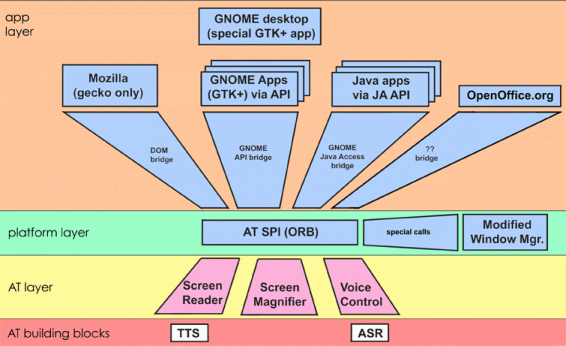
\includegraphics[width=1\textwidth]{obrazky-figures/GNOME_desktop_Accessibility.png}
	\caption{GNOME Accessibility Architecture overview\cite{gnomeADG}}
	\label{ATSPI_architecture}
\end{figure}

The widget is accessible, if a developer uses any GTK3/GNOME widget and follows the general accessibility guidelines\footnote{https://developer.gnome.org/accessibility-devel-guide/stable/gad-coding-guidelines.html.en} with properly implemented ATK interfaces. A newly developed widget, based on one of the stock GTK3/GNOME toolkit widgets, inherits the functionality and gains the accessibility support as well. The default implementation of the ATK interfaces might be altered by applications. Therefore, a developer can enrich their descriptions of widgets and improve the overall user experience in special cases, e.g. when a widget is used for some less expected purposes or the default description is too general. The ATK provides a set of functions to achieve this along with the ability to make any custom component accessible\footnote{https://developer.gnome.org/accessibility-devel-guide/stable/gad-custom.html.en}.\cite{accessibleWidgets}

\newpage
\section{Library Pyatspi}\label{library_pyatspi}
The package pyatspi is a Python wrapper around AT-SPI's C implementation, which loads the Accessibility typelib and imports the classes implementing AT-SPI interfaces.\cite{pyatspi}

AT-SPI exposes applications as a tree of widgets. On the top, the root element represents the whole GNOME desktop. Every sub-element represents one running application on the GNOME desktop. Each application has zero or more child elements, each child is distinguishable by its position in the tree and several object properties. Some of these properties are encapsulated inside the accessible object and their values must be obtained through corresponding methods, so-called \textit{getters}. A small set of properties are described in the following list:
\begin{itemize}
    \item \textit{name} - a string value, for most widgets contains text identical with a text label visible on a widget
    \item \textit{roleName} - a string value, specifies the widget type, available via \textit{getRoleName} method
    \item \textit{childCount} - an integer value, represents a number of sub-elements 
    \item \textit{actions} - a dictionary that contains available actions which can be performed on a widget by the ATK
    \item \textit{visible} - a boolean value, indicates that a widget is visible to the user
    \item \textit{showing} - a boolean value, a windget is rendered
    \item \textit{text} - a string value, mostly used in input fields or widgets containing plenty of text
    \item \textit{description} - a string value, contains a special widget description for users
    \item \textit{position} - an integer tuple, x, y coordinates on the screen (might be related to other component)
    \item \textit{size} - an integer tuple, shows the height and width of a widget
\end{itemize}

Additionally, the elements can be linked together in other useful ways (except the parent-child relationship), where the input widgets (e.g.: text field, check box, combo box, etc.) are linked with the elements that serve as their labels. These labels are making the input widgets easier to identify or interact with. Other advantageous element properties e.g. \textit{showing} or \textit{visible} are used to decide whether the element is hidden from the active screen area, thus it is not available for interaction. The \textit{roleName} attribute allows the categorization of widgets that is useful for identification of category-specific methods, e.g. selecting a radio button value, selecting an option in combo boxes, or a click method performed on push buttons. The access to the input functionality is focused in a singleton object named \textit{registry} that provides services for subscribing to specific events and generating  mouse or keyboard events on demand.

The library pyatspi is an open-source project available for most Linux distributions via distro specific packaging services (package named \texttt{python3-atspi}) or is available to be built from its sources\footnote{https://gitlab.gnome.org/GNOME/pyatspi2}.

\section{Exploring and Debugging The Accesibility}
Currently, there are several tools available for exploration and debugging accessibility features not only on the GNOME desktop.

\subsection{Dogtail}\label{sniff_accerciser}
Dogtail is an open-source GUI test framework written in Python and implemented as a library around the pyatspi. Several modules implement a higher level of API to simplify work and interaction with the accessible objects during the test development. The tool offers less complex functionality, containing tree view of objects with their basic attributes\cite{dogtail_doc}. 

The package dogtail also includes a GUI tool \textit{Sniff} (AT-SPI Browser on Figure \ref{sniff}), similar to the \textit{Accerciser} application described in the next section. The next paragraphs are dedicated to the description of the dogtail modules.

\begin{figure}[h]
	\centering
	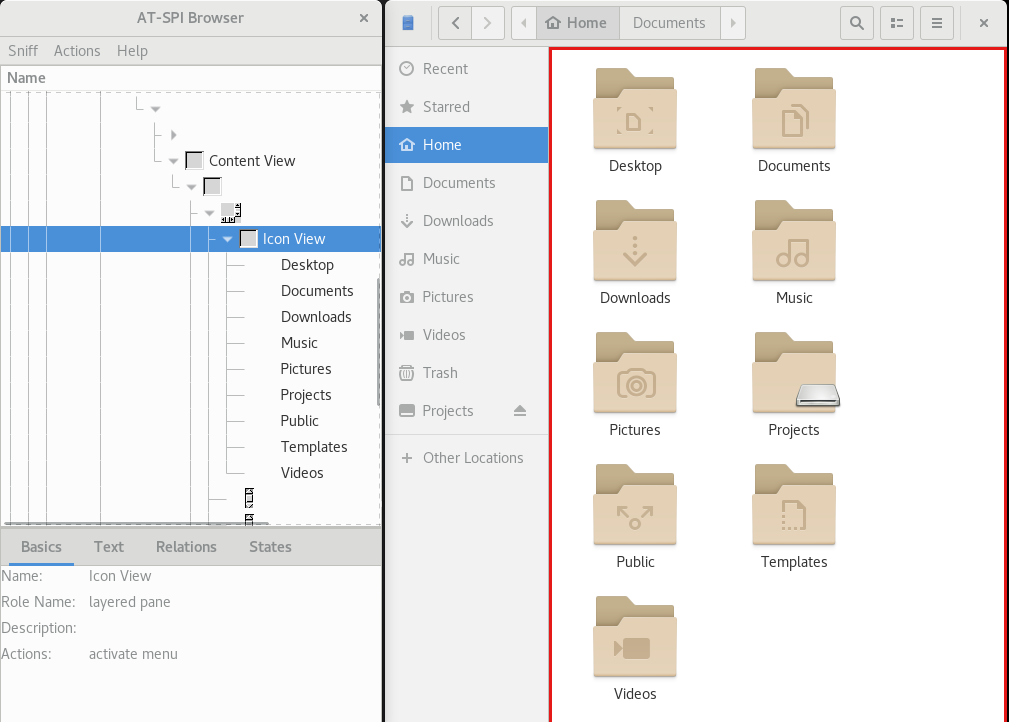
\includegraphics[width=0.9\textwidth]{obrazky-figures/sniff.png}
	\caption{Sniff utility (AT-SPI Browser), highlighting \textit{Icon View} area in \textit{Nautilus} file manager}
	\label{sniff}
\end{figure}

The module \texttt{tree} contains the most important class \texttt{Node}, instances of the class represent elements of the desktop user interface. All elements are gathered to the tree structure, representing all applications starting with the root element (desktop). The class is implemented as a mixin for Accessible and various Accessible interfaces and is an important unit for its subclasses, namely \texttt{Application}, \texttt{Root} and \texttt{Window}. The \texttt{Node} class also implements methods used for search of nodes in the tree based on certain criteria. A lambda expression can be passed to methods \texttt{findChild} and \texttt{findChildren} as argument named \texttt{pred}. The lambda expression can contain any properties that uniquely identify nodes, including \texttt{name}, \texttt{roleName},  \texttt{showing} and \texttt{visible}. The class also contains action methods that can be performed on nodes without importing other action modules. Verification and identification of shown nodes is easier thanks to the method named \texttt{blink}. Once the method is called on a certain element, the element is highlighted on the screen for several seconds. This functionality is also part of the Sniff tool where an element is highlighted after it is selected in the displayed tree.

The module \texttt{dump} contains only one method with the same name. The method returns a string describing the tree of nodes which is useful for python/ipython console debugging.

Finally, the module \texttt{rawinput} contains the implementation required for generating events from both keyboard and mouse. More complex events simulating keyboard shortcuts, mouse gestures, and drag and drop operations are implemented as well.

Testing Dogtail has proven availability for many Linux distributions through their package repositories, specifically Fedora 32, Red Hat Enterprise Linux 8.2 and Manjaro 18 with GNOME 3.34 (Archlinux). It is also available as a \textit{Pypi} Python package and according to information in it's official Gitlab repository should work not only for GTK3 application but also for application written in QT and KDE. 
 
Dogtail testing reveals some minor problems which might occur during the test development. There are known cases in which the coordinates of a node were not reported correctly. Most of the elements with the \texttt{roleName} value \textit{panel} and \textit{list box} are missing their \textit{name} values. Elements without the \texttt{name} value are much harder to identify, although they might not be important for users, as they don't contain any visible text, nor do they offer a way of interaction. The purpose of those elements is to serve as a wrapper that groups other elements together in a tree. 

Further testing discovered a non-accessible menu\footnote{https://bugzilla.redhat.com/1723836} or a nameless menu button\footnote{https://wiki.gnome.org/Apps/DiskUsageAnalyzer}. Once an action needs to be dispatched on such element, the identification has to be done either through a parent element or a sibling element. Additionally, the execution of a mouse event will require an offset calculation to specify the correct element position on the screen.
 
 So to conclude this chapter, dogtail is a powerful tool for the development of automated test cases in the GNOME3 environment. On the other hand, it contains discussed limitations and flaws. Those limitations must not come from dogtail itself, they are either accessibility bugs or bugs in the GTK3 framework (non-accessible menu).  

\subsection{Accerciser}
Accerciser is an interactive accessibility explorer developed in Python. It provides a well-arranged graphical frontend for the AT-SPI library, hence it can inspect, examine and interact with widgets. It also serves as a verification tool for developers, to check that their applications are providing correct information to assistive technologies and automated testing frameworks. Compared to Sniff, Accerciser's interface (Figure \ref{Accerciser_img}) offers extended features and functions. The default interface has three sections, a~tree view with the entire hierarchy of accessible objects and two optional plugin areas. The~Accerciser has an extensible, plugin-based architecture. Most of the features available by default are provided by plugins discussed in the next several paragraphs.

The \textit{Interface Viewer} plugin is an explorer of the AT-SPI interfaces provided by each accessible widget of a target application. When a tree element is selected, its interfaces are shown with a list of sensitive methods. The majority of methods are executable. The list contains methods for interaction with an object and various methods for obtaining more information about the object. Accerciser offers an exploration of the following interfaces:
\begin{itemize}
    \item Accessible - shows child count (number of child widgets), description, states, relations, and other attributes
    \item Application - if implemented (not mandatory), it shows application ID, toolkit and version
    \item Component - shows element's absolute position with respect to the desktop coordinate system, the relative position with respect to the  window coordinate system, size, layer type, MDI-Z-order indicating the stacking order of the component and alpha
    \item Document - shows document attributes and locale information
    \item Hypertext - shows a list with all element's hypertext links,  including name, URI, start index and end index
    \item Image - shows element's description, size, position and locale
    \item Selection - shows all selectable child items of the selected item,
    \item Streamable Content - shows selected element's content type and their corresponding URIs
    \item Table - shows element's caption, rows, columns, number of selected rows, number of selected columns and for the selected cell, it shows  it's row's and column's header extents  
    \item Text - shows selected element's text content, that can be editable with attributes offset, justification  and possibility to show CSS formatting as well
    \item Value - shows an element's value, minimum value, maximum value, minimal increment for a value 
\end{itemize}

\begin{figure}[hbt]
	\centering
	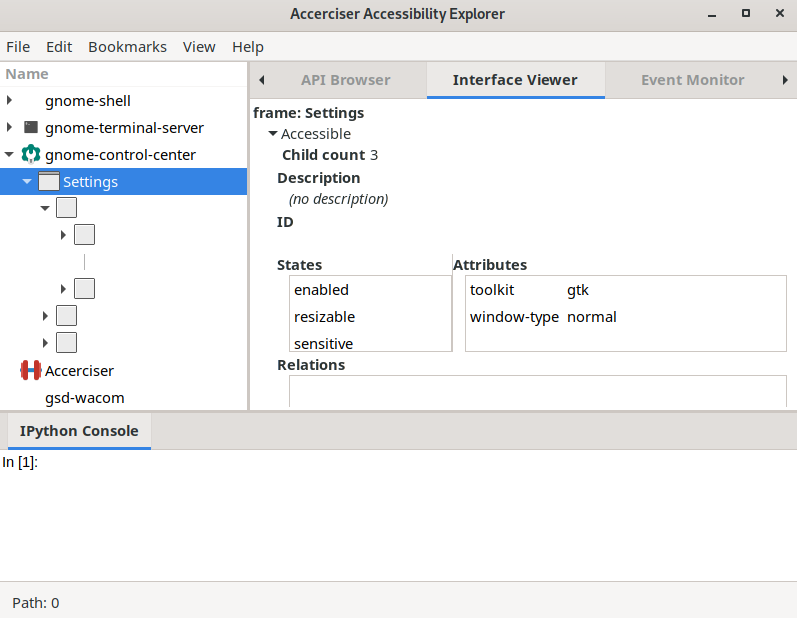
\includegraphics[width=0.9\textwidth]{obrazky-figures/accerciser.png}
	\caption{Accerciser's default configuration}
	\label{Accerciser_img}
\end{figure}

The \textit{AT-SPI Validator} plugin applies tests to verify the accessibility of a target application. The validator will generate the report of the selected item and all its descendant widgets in the tree hierarchy.

The next plugin is the \textit{Event Monitor}, which displays AT-SPI emitted events including the filter for several different AT-SPI event classes. The plugin has the ability to monitor only events sourced from the selected application or a selected accessible (widget). Each event record contains the source and the application.

The \textit{Quick Select} plugin provides global hotkeys for quickly selecting accessible widgets in the Accerciser's Application Tree View, the selected widget is highlighted in the target application.

The \textit{API Browser} plugin shows interfaces, methods and attributes available on each accessible widgets of a target application. By default, it shows only public methods and properties. Private methods and properties are hidden until checkbox \textit{Hide Private Attributes} is unchecked.
 
Finally, the plugin \textit{IPython Console} provides a full, interactive Python shell. The console has immediate access to any selected accessible widgets of a target application. The currently selected object in the tree view is available in the IPython Console under the symbol \textit{acc}. The plugin provides an easy way to test and debug code used in test cases.    
\section{Covering Limitations of Accessibility and Verification}
As discussed in the aforementioned sections, the information provided by accessibility is not flawless. Therefore, the next couple of chapters are dedicated to the exploration of technologies that might be used to support the accessibility in such cases.

\subsection{OpenCV and Image Matching Techniques}
OpenCV or Open Source Computer Vision Library is a software library that provides optimized algorithms for computer vision and machine learning. According to the official OpenCV webpage\cite{opencv}, the library contains more than 2500 algorithms and it is being developed 
by a vast community of contributors around the world. The library is used extensively bu government institutions, research groups, and companies including Microsoft, Google, IBM, etc. One of the biggest advantages is its native C++ implementation with bindings making the library available in Python, Java, and Matlab and supports Linux, Android, Mac OSX, and Windows. Regardless of Linux distribution, similarly to dogtail, OpenCV can be installed easily via python3 package manager (\texttt{pip}). 

From the rich availability of algorithms provided, the image recognition algorithm can be used to either locate or verify the presence of an element on the screen. This approach would require to have a set of images containing elements prepared in advance, then it can be used to find the image location on the screenshot of the screen taken during a test run. Compared to verification of the node only via accessibility, this approach would also verify that the element is properly rendering on screen and the shown result is an element that is shown to the user. An additional benefit is the verification of text formatting and colors. On the contrary, this process requires additional manual work of taking images, labeling them, and associating them with certain test scenarios. Count of elements displayed on the screen multiple times creates another parameter that would require manual maintenance. The most common example of such cases are buttons labeled either OK or Cancel as they are used in many applications.

Another possible approach is to use the shape recognition algorithm which can locate shapes like circles, rectangles, and many other common shapes. From the development perspective this would be easier to maintain, as there is no requirement for images prepared in advance. Frequent application changes during software development may also cause that tests based on image matching can be easily outdated. This factor forces testers to revisit test suites, therefore the efficiency of automated tests deteriorates. It can also help with the widget location in cases where accessibility is reporting wrong coordinates. On the other hand, locating the right widget in cases when several similarly shaped ones are located on the screen at the same time will yield very inconsistent results.

\subsection{OCR}\label{OCR_section}
The Optical Character Recognition or OCR is a method of extracting text from images. One of the available open-source tools is a tool called Tesseract.

Initially, Tesseract development started in 1985 at Hewlett Packard Laboratories but the major breakthrough was achieved in 2006 when the project was open-sourced in cooperation with the University of Nevada in Las Vegas. Since then, the project has been developed under the sponsorship of Google\cite{tesseract_history}.

Usability of Tesseract was increased in version 3.x, supporting a wide range of image formats and gaining the ability to be used in a larger number of scripting languages. While Tesseract 3.x is based on traditional computer vision algorithms, in the past few years methods based on Deep Learning have surpassed traditional machine learning techniques by a vast margin, especially in terms of accuracy in several areas of Computer Vision. Remarkable results were achieved in handwriting recognition. Tesseract has implemented a Long Short Term Memory (LTSM) based recognition engine which is a kind of Recurrent Neural Network (RNN). While this kind of RNN is used to recognize the text of random length, a Convolutional Neural Network is used just for recognition of single character. Version 4 provides both legacy OCR engine and new LSTM engine which is enabled by default.\cite{tesseract}

Tesseract can be used as a command-line tool, integration in development is possible via Tesseract's API available in python or C++. Setup on Linux or other platforms may differ but the process is accurately described in Tesseract's wiki\footnote{https://github.com/tesseract-ocr/tesseract/wiki}, with the last resort solution - building it from its sources.
The setup process includes installation of the \texttt{tesseract-ocr} package itself, \texttt{pytesseract} python bindings installable via python's package manager pip, and Tesseract's language pack with trained data for English language (version 4.x supports 130 languages\footnote{https://github.com/tesseract-ocr/tesseract/wiki/Data-Files\#data-files-for-version-400-november-29-2016}). 

Tesseract's OCR engine works best when used with images containing black text on white background in a common font. Text should be approximately horizontal with the height of at least 20 pixels. Surrounding borders around the text can be detected as some random text. With possibilities of image processing provided by OpenCV, the image quality in some cases needs to be improved before applying text detection methods. The most common image preprocessing methods include inverting images, rescaling, binarisation, noise removal, rotation, border removal, and page segmentation\footnote{https://github.com/tesseract-ocr/tesseract/wiki/ImproveQuality}.

Tesseract's API for python is bundled in a module named \texttt{pytesseract}. The module provides several methods, the most important ones for the purpose of this work are \verb|image_to_string| and \verb|image_to_data|. Both methods have one compulsory parameter which is an image intended for text extraction. An image has to be in a certain format, one of the options is to load the image through OpenCV's \texttt{imread} method. Additional parameters may be applied including language, timeout, and engine configuration\footnote{https://pypi.org/project/pytesseract/}. The first method returns all recognized strings including all whitespaces and other special characters. The second method provides additional metadata about all recognized strings in a form of dictionary-like object. The returned dictionary contains the following lists of properties:

\begin{itemize}
    \item text - string value, may contain a string, special character, one word or line of text
    \item left - integer value, specifies the number of pixels from the left side of the image 
    \item top - integer value, specifies the number of pixels from the top of the image
    \item width - integer value, specifies the width of the recognized string 
    \item height - integer value, specifies the height of the recognized string
    \item the rest are less important values for this work: \verb|level, page_num, block_num| \\ \verb|par_num, line_num, word_num, conf|
\end{itemize}

\begin{figure}[H]
	\centering
	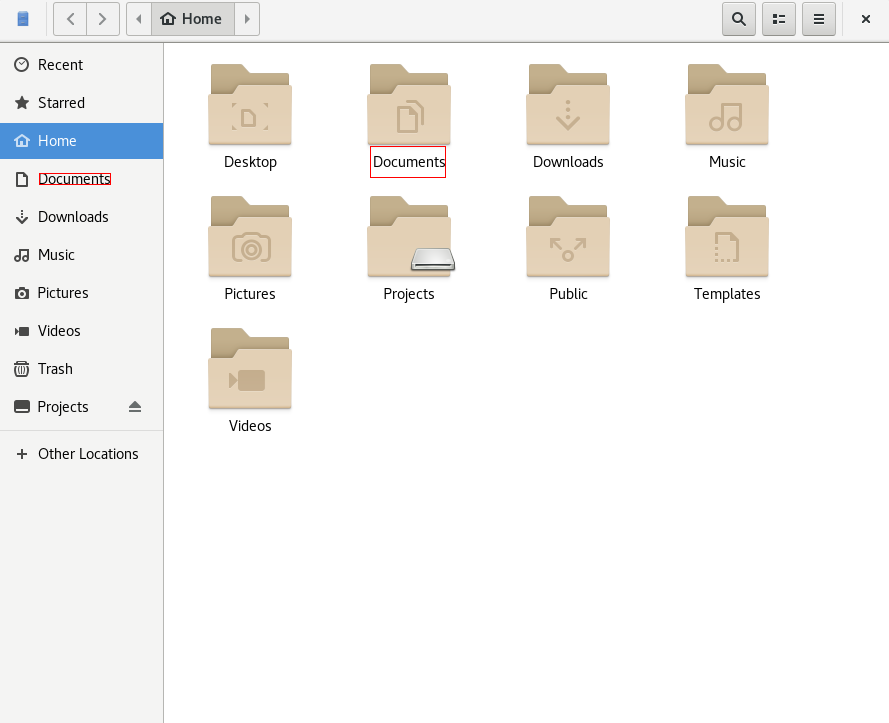
\includegraphics[width=0.9\textwidth]{obrazky-figures/ocr+nautilus.png}
	\caption{Demonstration of the OCR engine detection for the string Documents in Nautilus File Manager window}
	\label{ocr_nautilus}
\end{figure}

Figure \ref{ocr_nautilus} contains a demonstration of the Tesseract engine capabilities. The task was to locate the string \textit{Documents} in the screenshot of the GNOME file manager application \textit{Nautilus}.
The engine successfully found both strings located in the image and provided coordinates and dimensions that were used by OpenCV to highlight the strings in the image. 

Similarly to OpenCV, Tesseract's OCR engine was tested as an alternative tool for location or verification of widgets that contain text. This method also verifies that the content was properly rendered and is readable for the user. OCR systems have limitations and work with a certain margin of error which is a fact that also applies to Tesseract. Various applications can use different color schemes including background colors and font colors, input fields, and labels. Highlighting elements to perform actions on them can also lead to changes in color conditions. Image preprocessing methods provided by OpenCV can aid in avoiding problems associated with those cases, namely color inversion and binarisation. Those methods would supply Tesseract's engine with an image containing black text and a white background for evaluation.

\section{Conclusion}\label{ocr_conclusion}
This chapter has been dedicated to the Accessibility technologies in GNOME desktop with a deeper look at implementation, libraries, and tools for debugging. Furthermore, technologies that may be able to cover limitations and bugs in accessibility have been evaluated as well. Both OpenCV and Tesseract may help with identification, location, and verification of non-accessible elements in applications. A possible disadvantage is a delay caused by taking and processing screenshots of applications that have to be taken at the right time. OpenCV's image matching algorithm can reliably locate prearranged images of icons, labels, or whole application windows on the screen. Considering the stable application environment with black text on white background in most applications, Tesseract can detect and reliably locate most of the text content on the screen. Other cases can be covered by image preprocessing done again in OpenCV. Both technologies are working with actual application content rendered to users, possibly bringing an additional level of verification. However, the goal of this work is to generate test cases dynamically and preparation of a set of screenshots to verify a proper rendering of icons would violate this effort. A possible solution could be to take screenshots during the test generation process. However, an icon would need to be cropped out from the screenshot, thus relying on the position if the icon reported by the AT-SPI. Therefore, an integration of the Tesseract's OCR would be more beneficial for this project.

\chapter{Proposed solution}\label{proposed_solution}
A goal of this work is the development of a tool with the ability to generate automated test cases for GUI applications. The proposed test generator works with the AT-SPI metadata provided by applications and converts them to test cases. The required metadata should be available for a lot of applications, assuming they are developed in one of the common frameworks (GTK3, QT). However, this tool is focused on applications for GNOME desktop\footnote{https://wiki.gnome.org/Apps}. A tool will be developed in language Python3, version 3.6.

All applications are open source and are developed by the community of enthusiasts around the GNOME project. Anyone from the community can fix bugs in applications by sending a merge request with fixes, request a new feature, or propose newly developed features. This development model does not contain a planning phase or a phase where one can design an abstract model of an application, from which test cases could be derived. Therefore, the solution is based on the derivation of the model from the AT-SPI metadata. The extracted data about widgets and relationships between them, provides the foundation which gives the test generator the ability to interact with an application. Therefore, the test generator can use the extracted information to perform the exploratory testing. The testing includes execution of the scenarios (or so-called \textit{test sequences}), monitoring the behavior of the SUT, and detection of certain errors and crashes of the SUT. The test cases are generated as a by-product of this process.

\begin{figure}[hbt]
	\centering
	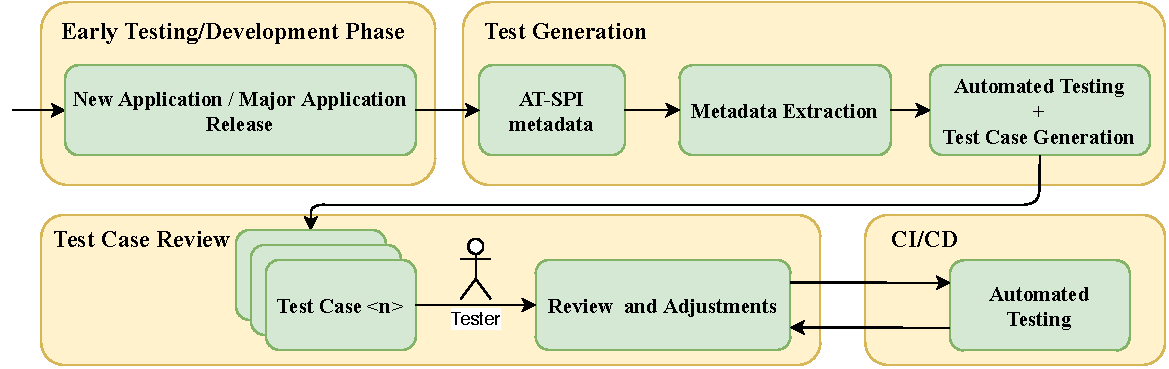
\includegraphics[width=1\textwidth]{obrazky-figures/overview.pdf}
	\caption{Architecture of the proposed solution}
	\label{Diagram}
\end{figure}

Figure 4.1 describes an overview of the workflow with the proposed test generator. The beginning of the scenario starts with either a newly developed application or a version of an application that contains major changes. The tool should perform initial exploratory testing of the application based on the extracted model and export those scenarios in the form of \textit{behave} test scenarios.

From the testing perspective the proposed tool combines several testing techniques. The extracted AT-SPI metadata creates the foundation for a simplified model of the application by partially adapting the model-based testing technique. Since the test cases are derived from the model without any knowledge about the implementation of a tested application, the tool resides in the category of black-box testing. The knowledge about the SUT provided by the model allows the tool to benefit from the approaches described in the random input testing and random walk tools in a more deterministic way. The tool can be characterized as a semi-smart tool as it can detect certain crashes of the SUT during the test generation and immediately report them with a reproducer. The results of the test generation process are test cases that may be adjusted and executed again. The tests are executable in the CI/CD pipeline that can be triggered at any stage of the application development and report the results without manual retesting.

\section{Model Extraction}
The model created as an abstraction of a test application is described as follows: 

\theoremstyle{definition}
\begin{definition}
A Model $M$ is a 4-tuple: $M = (N, E, S, T)$ (a directed graph), where:
\begin{enumerate}
\item $N$ is a finite set of $Nodes$ (widgets associated with an executable action, or a root element);
\item $E$ is a finite set of $Events$ (actions), where  $E\ =\ \{e\ |\ (n_S, e, n_T)\ \in\ T \land\ n_S,n_T\ \in \ N\}$;
\item $S$ is a set of starting $Nodes$ (a root window element)  $S\ \subseteq\ N\}$;
\item $T\ \subseteq\ Node\ \times \ Event\ \times \ Node$ is a transition relation.
\end{enumerate}
\end{definition}

The model extraction process relies on the AT-SPI metadata that is provided after the start of an application. As mentioned in section \ref{library_pyatspi}, once the application is running, a tree of widgets is exposed and available for interaction. The provided representation of the tree itself is not suitable to be directly used as a model of an application, as the implementation contains several restrictions for purposes of this work.

The first restriction is represented by nodes/widgets with no functionality nor a way of interaction for the user, e.g.: filler, separator, panel, etc. Theoretically, a copy of the three could be created with those nodes filtered out, although in that case the parent-child relationship in the tree needs to be restored accordingly. This is not possible, since the attributes \texttt{children} and \texttt{parent} in \texttt{Atspi.Accessible} object instances are read-only. 

The tree also contains references to properties and methods which are available only during application runtime and possibly disallowing access to the properties of an extracted model after application crashes or terminates. Furthermore, the test generator must start the execution of every test scenario (test sequence) from the default state which is achieved by obtaining a fresh instance of a tested application.

Additionally, the custom implementation of the model allows us to track the progress of the test generation process. The model consists of objects gathered in test sequences, each object has its unique identity that lasts throughout the test generation process. This implementation allows us to measure the event coverage and ensures that an already executed test sequence is never repeated.

A solution for those restrictions is a custom implementation of the accessibility tree. In the beginning, a custom tree is derived from the original tree provided by the \textit{dogtail}. The unusable nodes are filtered out, while the parent-child relationships of the nodes are preserved. The custom tree can be used as a model, that will map the possibilities of interactions available for users working with an application. The model includes every node from the original tree with available actions that are also executable by the AT-SPI.

The development revealed, that not all rendered widgets are properly labeled with actions by AT-SPI. To be specific, nodes with role names \texttt{page tab} and \texttt{list item} are not labelled with actions. The first mentioned has to be clicked to gain access to additional nodes, the second one can be placed on the same level as a push button. Therefore, the generator relies on records in file \texttt{roleNames.py} where the role names of actionless nodes are enumerated. If a node is not associated with any action, the default action for the node is \texttt{click}.

However, the model does not allow the execution of the actions directly, as the generation process requires to run several instances of an application. The instances of accessible objects and some of their properties are valid only for one application runtime. Therefore, several important values are extracted in the process, making them available even after the termination of an application instance. The properties \texttt{name, roleName, parent\_name, parent\_roleName} are used as the unique identifier because some nodes might share the same \texttt{name} and \texttt{roleName} (e.g. OK, push button). The properties give the test generator the ability to match each node from the model to the current application instance exposed by the accessibility. The implementation of the model is presented in the class diagram in Figure \ref{tree_diagram}.

\begin{figure}[hbt]
	\centering
	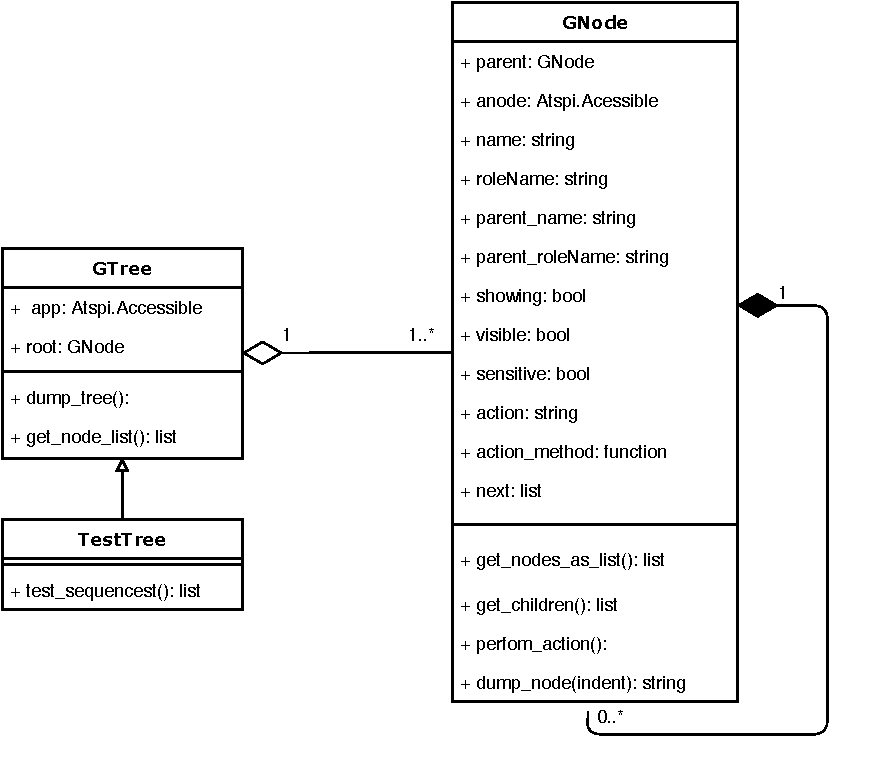
\includegraphics[width=0.8\textwidth,clip]{obrazky-figures/tree_diagram.pdf}
	\caption{Class diagram of the model}
	\label{tree_diagram}
\end{figure}

Starting from the lowest level, an instance of the class \texttt{GNode} represents one node from the tree. Several attributes are copied from the original \texttt{dogtail.tree.Node} instance, including attributes storing the pieces of information about the parent node, the data describing the state of the node, the list of children, and if available, the name of the action method. The list of children is also composed of instances of the \texttt{GNode} class, so the tree is recreated recursively. Therefore, the model can hold all information about tested applications, without relying on their state. An instance of the \texttt{GTree} can represent either a whole application or a smaller part of the application e.g.: a dialog or a menu. As discussed previously, this offline model of the application tree also contains a lot of nodes without the ability of interaction, which needs to be filtered out. Those nodes are identified by the list of \texttt{RoleName}s that are gathered in the separate file \texttt{rolenames.py}. Finally, the class \texttt{TestTree} serves as a wrapper that filters those nodes and preserves the parent-child relationship. The result of this process is an instance of the \texttt{TestTree} object and it contains only nodes required to generate test cases. 

\section{Test Environment}
Before the generation process starts, it is necessary to have the implementation for monitoring the state of tested applications and acquire the ability to perform start and stop operations. The test generation process performs various actions available in an application that might change settings or layout of the application. Generation of every test case must start from the same state which should satisfy the following conditions: 
\begin{enumerate}
    \item an application is not running, if so, force the application to stop
    \item reset the application's settings to the default state by performing predefined custom cleanup
    \item start a new instance of the application with the default settings.
\end{enumerate}

\subsection{Test Environment Setup}
The test case generation process depends on the execution of applications in the GNOME Shell desktop environment. The environment contains various features\footnote{\url{https://help.gnome.org/users/gnome-help/stable/shell-introduction.html.en}} like workspaces, notifications, the application grid, the activities overview, and menus, that can be triggered either via mouse or keyboard. Those actions can bring the environment to multiple states. Execution of an action that brings the environment to some of those states takes the focus from the tested application back to GNOME Shell, thus blocking any further interaction. A notification might collide with the user interface of the tested application and block the execution of an action during the test case. These factors need to be avoided to ensure stability during the test generation and the test execution as well. The setup must also be able to recover the environment from potential test case failures and will not influence the execution of the subsequent test cases. 

The required setup for the test execution is implemented in the module \textit{qecore}. The module is designed for test automation of GNOME desktop applications and contains various measures designed to avoid occurrences of unintentional environment events and focus on a tested application. The module is bound to \textit{dogtail} and it is intended to be used with \textit{behave} framework.\cite{qecore} 

The test generation process partially relies on the provided setup. However, a different approach is used in terms of monitoring tested applications. For this reason, a custom class \texttt{App} is derived from the qecore's \texttt{Application} class. Throughout the development of the test generator, the implementation of the \texttt{App} class diverged, and the majority of the implemented methods were rewritten. Although, the \textit{qecore's} \texttt{Application} class is still being used for the test case execution. The inheritance acts as a safeguard that makes sure that provided data about tested applications are sufficient to create an \texttt{Application} instance. Or in other words, it serves as an assertion that generated tests will be executable before the generation process starts. The relationship between classes is shown in Figure \ref{test_gen}. The test generator integration with the \textit{qecore} led to contributions that were delivering minor fixes\footnote{\url{https://gitlab.com/dogtail/qecore/-/merge_requests/24}}\textsuperscript{,}\footnote{\url{https://gitlab.com/dogtail/qecore/-/merge_requests/26}}. Another contribution\footnote{\url{https://gitlab.com/dogtail/qecore/-/merge_requests/25}} submitted an implementation of the new attributes for the \texttt{Application} class to solve the problem with location of desktop files required to test LibreOffice applications.

\subsection{Test Environment Configuration}\label{env_config}
Assurance of compatibility with various applications across the GNOME ecosystem requires that some metadata describing the tested application has to be provided before the test generation process. The metadata is gathered in a configuration file written in YAML\footnote{\url{https://yaml.org/}} language and only contains the most necessary information required to recognize tested applications. The reasons behind choosing YAML is syntax simplicity and human readability in comparison with e.g. JSON\footnote{\url{https://www.json.org/json-en.html}} or XML\footnote{\url{https://www.w3.org/XML/}}, followed by the reliable support in Python provided by library \texttt{pyyaml}.\cite{yaml} The  configuration file serves as a single source of truth for the test generator. All changes in the medatada required to test the application are done within this file, thus avoiding any changes in the source code of the test generator.

\begin{lstlisting}[language=yaml,caption={Example of the apps.yaml entry for LibreOffice Start Center},label={apps.yaml}]
libreoffice-startcenter:
  a11y_app_name: soffice
  app_process_name: soffice.bin
  desktop_file_path: /usr/share/applications/libreoffice-startcenter.desktop
  kill_command: "pkill soffice"
  params: "--norestore" # required to avoid unwanted file restore dialogs
  cleanup_cmds:
    - "pkill soffice" # LO required a custom kill cmd
    - "rm -rf .config/libreoffice/*"
  packages:
    - libreoffice
  flatpak: False
\end{lstlisting}

The \texttt{apps.yaml} gathers data about all tested applications. Each application entry starts with an application name on the top level. The application name should be unique as the name is used as a folder name of the generated project. Required values may vary per tested application. Some of them might not be necessary for the test generation, although they are required for the test execution.

The list of items that can be defined for each application includes:

\begin{itemize}
    \item \texttt{a11y\_app\_name} - is the only compulsory item, it defines a name of the application in the accessibility tree, the value can be found in GUI tools Sniff or Accerciser as previously discussed in Section \ref{sniff_accerciser}, the value can match with the name of the application
     \item \texttt{app\_process\_name} - is required if the name of the application process differs from the application name, the value is used during the cleanup in between the executions to make sure that an instance of the application has been killed and a next test will use a new one
     \item \texttt{desktop\_file\_path} - required if default qecore's method fails to find the desktop file of an application, the desktop file contains useful data about applications, including a command required to run an application from the command line
     \item \texttt{params} - required if the application needs to be run with custom command line parameters, all parameters should be entered in one string, separated with a space
     \item \texttt{cleanup\_cmds} - if provided, contains a list of commands that will be executed after the generation of each test case. Executed commands should always restore the application to its default settings. The commands are also used during the test execution of generated test cases, after finishing each test case. 
     \item \texttt{packages} - required for execution in the CI environment, contains a list of rpm\footnote{https://rpm.org/} packages required to be installed to both generate and execute tests
     \item \texttt{flatpak} - required if a tested application is a flatpak
\end{itemize}

\subsection{Flatpak Applications Setup}
Flatpak\footnote{\url{https://flatpak.org/}} is a technology for building and distributing desktop applications on Linux. Flatpak aims to solve the problem with the cross-platform distribution of packages on Linux, thus avoiding problems with different package managers used across Linux distributions. Applications, or so-called flatpaks, are delivered to users regardless of the lifecycle of the underlying Linux distribution. The system implements a set of sandboxing technologies, to isolate flatpaks from each other and the system, thus providing security benefits to users.\cite{flatpak}

The majority of GNOME applications are also available through flatpak. A dedicated flatpak repository \textit{Nightly GNOME Apps} contains the latest development versions of GNOME applications. With Flatpak, those applications are installed alongside their stable versions. This gives us the potential to test the application much sooner before it is released to distributions. This is a benefit behind the integration of flatpak support to this work. The main repository for flatpak applications called Flathub\footnote{\url{https://flathub.org/home}} contains hundreds of applications developed in various frameworks and programming languages. However, the effort done by this work only supports applications developed in GTK3 as they obtain the accessibility support by design.

There are several differences in the runtime perspective between flatpaks and non-flatpak applications. Each application has a unique name, e.g.: \texttt{org.gnome.gedit}. The unique name is required for every operation executable through the \texttt{flatpak} command-line utility. The utility not only serves as a package manager able to install, remove, downgrade and update flatpaks, it also provides a sandbox to run flatpaks. Those differences demand certain changes in the runtime used for the test execution and the test generation. 

Considering the test execution, the approach used in the \textit{qecore's} \texttt{Application} class should be suitable for testing flatpaks. However, the initial testing emphasized the previously mentioned differences and it led to the conclusion that a separate class \texttt{Flatpak} has to be developed to achieve the same goals. The \texttt{Flatpak} class inherits the methods from the \texttt{Application} class and reimplements some of them do address those differences. The most important changes are:

\begin{itemize} 
    \item \texttt{\_\_init\_\_} - the constructor performs a validity check on inserted flatpak ID, the format requires two dots, e.g. \texttt{org.gnome.gedit}
    \item \texttt{start\_via\_command} - runs a flatpak via only via command and with the flatpak command-line utility, e.g. \texttt{flatpak run <id>}
    \item \texttt{kill\_application} - terminates a flatpak via command e.g. \texttt{flatpak kill <id>}
    \item \texttt{get\_desktop\_file\_path} - performs a recursive search for flatpak's \texttt{.desktop} file in two possible locations:
    \begin{itemize}
        \item \texttt{\textasciitilde/.local/share/flatpak/app/} - flatpak installed per-user
        \item \texttt{/var/lib/flatpak/app/} - flatpak installed system-wide
    \end{itemize} 
    \item \texttt{is\_running} - performs a check if a flatpak is running, this is again done with the flatpak command-line utility (e.g. \texttt{flatpak ps <id>}) and the presence of an instance in the accessibility tree
\end{itemize}

Additionally, the invocation of some of the inherited methods does not make sense for flatpak applications. The invocation of those methods with an instance of the \texttt{Flatpak} class raises an exception. The exception contains a message with an explanation that the methods are not available for Flatpak objects. The developed changes were submitted to the \textit{qecore} projekt{\footnote{\url{https://gitlab.com/dogtail/qecore/-/blob/master/qecore/flatpak.py}}}.

On the test generator level, a new class \texttt{FlatpakApp} was implemented to manage the runtime of the flatpak applications. As described in the class diagram shown in Figure \ref{test_gen}, the \texttt{FlatpakApp} serves as a wrapper for the \texttt{Flatpak} class in the same manner as the \texttt{App} class wraps the \texttt{Application} class. \texttt{FlatpakApp} and \texttt{App} are customized classes for the test generator, while \texttt{Flatpak} and \texttt{Application} are used during the text execution. 

\subsection{Monitoring an Application State}
Several indicators can be monitored while the application is being tested. The most essential one is to be able to safely determine if the application is running at the moment or not. This can be done either by examination of the \textit{pid} (process id) belonging to the application process or by relying on AT-SPI. If the application tree is not available, it can be certainly assumed that the application instance is not running. This statement also applies vice versa, so an assertion that an application has started is achievable in the same way. The implementation takes advantage of \textit{dogtail's} \texttt{Tree.Node.Applications()} call, returning a list of applications currently exposed to the accessibility bus.

Furthermore, it is also necessary to perform certain checks during the time an application is being interacted with. Therefore, every tested application will be run as a sub-process, which enables us to capture the output generated by tested applications to standard streams (\textit{stdout, stderr}). Once an application has been terminated, it also allows us to check the return codes. The implementation relies on Python's standard library \texttt{subprocess}. 

The output generated to the standard stream is checked for errors defined in the designated configuration file. In case of error throughout the generation process, an error message is printed immediately to warn about the possible bug in tested applications. The warning contains the number identifying the test in which the error occurred, a full error message, and a return code. All other captured messages e.g. warnings or deprecation messages from the GTK framework are saved to one log file, in a folder where the tests are generated. The messages are being appended, so the log file can be checked at any time during the generation process. Every line contains the test number, so it can be easily determined when the message occurred and match it with the reproducer from the given test case.

The implementation of monitoring for the non-flatpak applications is encapsulated in the class \texttt{App}. The class \texttt{FlatpakApp} achieves the same goals for the flatpak applications.

\begin{figure}[H]
	\centering
	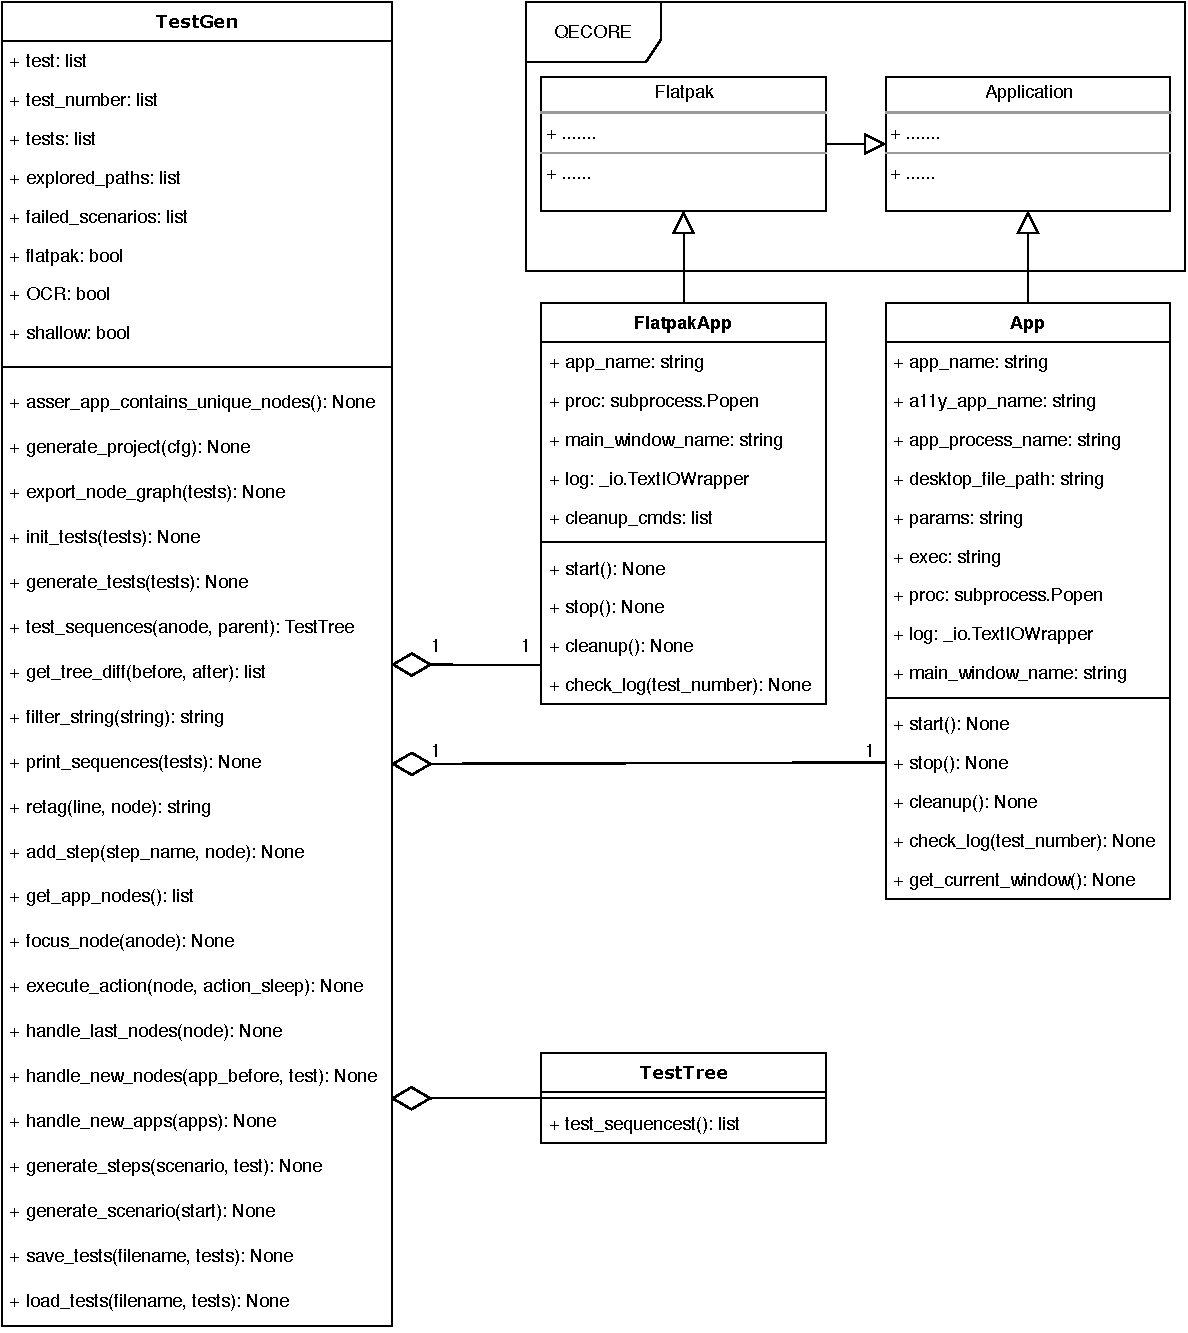
\includegraphics[width=1\textwidth,clip]{obrazky-figures/TestGen_class_diagram.pdf}
	\caption{Class diagram describing an overview over the implementation of the test generator}
	\label{test_gen}
\end{figure}

\newpage
\section{Generating Environment for the Test Execution}
The input of the test generator is provided by the data in \texttt{apps.yaml}. The output is a project structure containing generated test cases and other files required for the test execution. 

Initially, the test generator checks the availability of the entry for a tested application in the configuration file \texttt{apps.yaml}. Subsequently, it creates a sub-folder with the name of the application where generated content will be placed. Predefined source files with the implementation of \textit{steps} (used by \textit{behave} framework) are copied to the folder structure along with scripts and other files that are necessary for the test execution. Figure \ref{project_folder} demonstrates the structure generated for the application \textit{GNOME Terminal}.

\begin{figure}[H]
\dirtree{%
.1 gnome-terminal.
.2 features.
.3 generated.feature.
.3 environment.py.
.3 steps.
.4 ocr\_steps.py.
.4 steps.py.
.2 gnome-terminal.log.
.2 mapper.yaml.
.2 requirements.txt.
.2 runtesh.sh.
.2 cleanup.sh.
}
\caption{The generated project structure for the application \textit{GNOME Terminal}}
\label{project_folder}
\end{figure}

The sub-folder named \texttt{features} contains files with the \textit{behave} test cases. Test cases generated by the test generator are in the file \texttt{generated.feature}. The file contains a single so-called \textit{Feature} that contains all generated test cases. Test cases are composed of a tag, a brief description of the test case, and so-called \textit{steps}. The tag is a unique identifier of the test case and thus allows single test case execution, if required. The description should briefly define what should be done with the SUT, when the test case is executed. The steps are one-line statements, each of them describes either an execution of an action or an assertion described in a human-readable language. Successful execution of all steps evaluates the test case as passed. Otherwise, the result of the test case is a fail.

The file \texttt{environment.py} contains the setup required for the test execution. It contains 3 functions used by the \textit{behave} framework to set up or restore the required environment during the test execution. 

The \texttt{before\_all} function is run once before the execution of the test cases. It initiates the GNOME environment setup from the \textit{qecore} library and creates an instance of either the \texttt{Flatpak} or the \texttt{Application} class. The type of the application and the parameters for the class instance are extracted from the entry in the configuration file \texttt{apps.yaml}. 

The \texttt{before\_scenario} function is executed before every test case (scenario). It contains an invocation of the method from the \textit{qecore} that should set the testing environment to the default state and other preparations for the testing. Additionally, it executes the \texttt{cleanup.sh} script with a custom per-application cleanup defined in \texttt{apps.yaml} (discussed in Section \ref{env_config}). 

The \texttt{after\_scenario} function is called after the execution of every test case, regardless of its results. The result is then submitted to the generated test report.

The folder \texttt{steps} contains source files with the implementation of the \textit{steps} used in the \textit{behave} scenarios. The implementation of steps is divided into two files. The module \texttt{ocr\_steps.py} contains only one \textit{behave} step which encapsulates the implementation and optimization used for the verification of the string on the screen. The module \texttt{steps.py} contains general implementation of steps. The steps are functions implemented in Python with the \texttt{step} decorator from the \textit{behave} framework. The decorators serve as a wrapper to call the Python functions from the \texttt{.feature} files. So in the case of this project, the steps written in the test cases are function calls, the functions are defined in these modules. The definition of the \texttt{@step} decorator (Code Listing \ref{step_definition}) contains variables, thus allowing us to keep the code base as minimal as possible.

\begin{lstlisting}[
style=mypython,
caption={The implementation of the step that is used to make an assertion on any of the node's property},
label={step_definition},
  frame=tb,
  numbers=left
]
@step('State: "{roleName}" "{name}" "{prop}" is "{state}"')
def assert_state(ctx, name, roleName, prop, state):
    node = ctx.app.instance.child(name, roleName)
    focus_node(node)
    assert hasattr(node, prop), f'Obj: {node} is missing attribute {prop}'
    prop_value = f'{getattr(node, prop)}'
    assert state == prop_value, f'Expected: {state}, Got: {prop_value}'
\end{lstlisting}

The file \texttt{gnome-terminal.log} aggregates log messages produced by a tested application throughout the test generation process. The log file name is derived from the application name defined in the \texttt{apps.yaml} file. The \texttt{mapper.yaml} file contains a list of test cases with other data required for the CI execution. The file \texttt{requirements.py} contains all Python dependencies that need to be installed to execute the test cases. Finally, the \texttt{runtest.sh} is a wrapper script for execution of test cases.

\section{Test Case Generation}
The test generator implementation is encapsulated in the class \texttt{TestGen} (class diagram in Figure \ref{test_gen}). The behavior of the generator can be also influenced by several command-line arguments that will be described later in this work. Based on the parameters (\texttt{flatpak} item in \texttt{apps.yaml}), the instance of either the \texttt{App} or the \texttt{FlatpakApp} is created. 

The generator then creates a copy of the default project structure and injects the files inside the project structure with values that correspond to the application that is going to be tested (Figure \ref{project_folder}). Namely, the files \texttt{environment.py}, \texttt{mapper.yaml}, and \texttt{cleanup.sh} contain placeholders (tags) that are replaced by values defined in \texttt{apps.yaml}. Just note that no Python code is being generated during the process. The default project already contains all the predefined \textit{behave} steps required to execute generated test cases.
The next sections are dedicated to the details of the generation algorithm. The Algorithm \ref{test_gen_algorithm} contains a shorter version written in a pseudocode. 

\begin{center}
\begin{algorithm}[H]
\caption{Test generation algorithm pseudocode}
\label{test_gen_algorithm}
\SetAlgoLined
\KwData{Running application exposed to the accessibility bus, \texttt{apps.yaml}}
\KwResult{Test Cases}
 start the application\;
 scan the application tree, generate the test tree\;
 derive the test sequences\;
 terminate the application\;
\SetKw{KwInn}{in} 
 \ForEach{$sequence$ \KwInn $test\_sequences$}{
 application cleanup, if required\;
 start the application\;
  \ForEach{$action$ \KwInn $sequence$}{
   save the state before the action is executed\;
   execute the $action$\;
   add the action step to the test case\;
  \eIf{application is not running}{
   check return code and the logs\;
   \eIf{application crashed}{
    print reproducer and log\;
    }{
    add the quit assertion to the test case\;
    }
   }{
   evaluate the tree changes through the symmetric difference\;
   \uIf{action started new application}{
    generate the assertion\;
    }\uElseIf{action generated new window/s}{
    \ForEach{$window$ \KwInn $windows$}{
        append new sequences for the $window$\;
    }
    }\Else{
     append new sequences for new nodes\;
    }
  }
 }
 }
\end{algorithm}
\end{center}

% duplicit node renaming
\subsection{Derivation of Test Sequences}

The generator proceeds with a first start of a tested application and extracts the AT-SPI tree of the application instance through the \texttt{dogtail}. Then, a writable copy of the tree is created through the \texttt{GTree} instance. The action-less nodes are then removed and the remaining notes are placed in the new instance of the \texttt{TestTree} class. Test cases are derived from the test tree through the class method \texttt{test\_sequences}. 

The method returns a list\footnote{\url{https://docs.python.org/3/tutorial/datastructures.html}} with test sequences. A test sequence contains a list of nodes with actions that will be executed for every test case. The method gathers the list of leaves in the \texttt{TestTree}. Then it iterates through the list of leaves and calculates path from a leaf to the root of the tree. Each path contains a list of nodes. The result is a list of paths or as mentioned earlier test sequences. A test sequence does not represent a whole test case. The whole test case is created by applying the test sequence on the live instance of the application. While applying the test sequence, the generator appends assertions steps and OCR checks. The checks are generated either before or after the execution of actions and they will be used as a verification in a generated test case to confirm that the application reached the intended state. A test sequence can be used multiple times or it can be extended, if the generator discovers that the applied sequence led to a discovery of new nodes. Those new nodes are evaluated and the generator creates new test sequences, each of those sequences start with a sequence that led to their discovery. 

\subsection{Execution of Test Sequences}
The initial phase is completed by the termination of the application instance, the generator continues with the execution of test sequences (line 8 of Algorithm \ref{test_gen_algorithm}). From this point the generator works with 3 instances of the tree: the current running application instance obtained through \textit{dogtail}, the instance of the class \texttt{Gtree}, the instance of the class \texttt{TestTree} or so-called model used to derive the tests.
% online testing
% graph
The test generator then starts to iterate over the extracted test sequences, monitors the application, executes actions, and generates steps and assertions that are then put together in \textit{behave} scenarios. 

Every iteration of the test sequences works with a newly started instance of the application, so every scenario begins with a step that starts the application. The step internally contains an assertion to make sure that the application has started and is ready for the interaction. The generator stores a shallow copy of the list containing the applications that are currently available through AT-SPI. It also saves a copy of the currently available nodes in the tested application. 

The generator selects the first node from the sequence and locates the node within the currently running instance of the application. In case that application contains too many nodes (widgets), some of them might be hidden. The generator tries to avoid that by using \texttt{grabFocus} method on the node. The method does not work for menus, where the \texttt{select} method has to be used instead.  Additionally, the \texttt{node.sensitive} property is checked. If the value of the property is \texttt{False}, the generator prints a warning as the value indicates that the action might not be executable in the current state. Then the action associated with the node is executed. If the execution of the action was successful, the event coverage is increased and a step with the description of the node and executed action is added to the test scenario. The execution of the action is followed by several checks performed on the current instance.

Initially, the generator checks whether the application is still running by retrieving the application instance from the accessibility tree. If the application instance is no longer present, there are two possibilities. The application was intentionally terminated by the executed action or the application crashed. The decision is made by the examination of the generated logs (\textit{stderr, stdout}) and the value of the return code retrieved after the termination.

If the application was terminated with the return code value of 0, the test generator appends a new step to the test case. The step contains an assertion that the application is no longer running (Quit/Exit button). 

If the return code does not contain the value 0, the generator raises the error, prints the reproducer, the return code value, and the content of the obtained logs. The generator proceeds to the next test case. 

In some cases, the occurrence of an error does not mean that the application crashes. Therefore, the generator checks the log for known errors after every executed action regardless of the state of the application. The list of the messages that are being checked is stored in the file \texttt{errors.py}. A new error message can be appended to the list at any time. The list currently contains messages that previously occurred in bugs related to \textit{GNOME} applications.

\subsection{Model Expansion}
Successful execution of the action, followed by no errors detected in the log and application still being run, indicates that the action could have changed the state of the application. 

Initially, the generator checks whether the action triggered the execution of a new application. The detection is achieved through the symmetrical difference computed on two sets. The first one contains the list nodes representing running applications before the action was executed, the second one holds the list of applications available after the execution. Both lists are shallow copies, so the generator does not need to compare an entire tree for each application. If that is a case, the generator appends the assertion implying that the applied sequence led to the start of a new application. The test generator does not expand the nodes of the newly spawned application to the current test tree as they do not belong to the application that is currently being tested. This solution has limitations, an application that is not exposed to the accessibility bus will not be detected.

If the previously described effort failed, the generator proceeds to search for the changes within the tree of the tested application. The implementation takes advantage of the method \texttt{get\_node\_list} from the class \texttt{GTree}. The method returns all nodes from the tree instance in one \textit{list}. The list is converted to a set, and similarly to the process of detection of a new application, it calculates the symmetric difference between sets captured before and after the executed action. 

The generator distinguishes between several roles of the discovered nodes. The appearance of a new window or a dialog causes the generation of an assertion to the current test case. Regardless of a role, the generator creates a \texttt{TestTree} instance with new nodes (a subtree) and retrieves test sequences derived from the subtree. The new test sequences are prepended with the sequence that led to their discovery and then added to the list of the test sequences that will be executed in the next iterations.

The expansion during the test case generation can significantly increase the execution time. The test generator implements an option \texttt{{-}{-}shallow} that disables the expansion and generates test cases only from the model obtained from after the start of the application. The option gives testers the ability to obtain fundamental test cases that can be reviewed and updated in a much shorter time.

\subsection{Generating Reports}

\section{OCR integration}
The main goal of the OCR integration in this work is to provide an additional level of verification of string values presented by applications and thus not rely purely on AT-SPI. However, the integration of OCR into the generated test cases has to be reliable to avoid false-positive test results. For the reasons mentioned in \ref{ocr_conclusion}, the integration of OCR has to be properly tested, the implementation has to contain image preprocessing optimizations and configuration to achieve stable results. Tesseract offers several options that allow to optimize string detection and text analysis. One of them is the definition of the recognized language. It is assumed that most of the tested applications will use the English language and therefore, the dataset trained for the English language is used.

\subsection{Screenshot Preprocessing and Optimizations}
As discussed in \ref{OCR_section}, Tesseract is less prone to errors when operating with images containing black text on a white background. Therefore the safest option, is a conversion of images with thresholding to binary colors (black and white). It also has to be considered that some applications are using darker color themes or contain parts with different color schemes. To avoid problems with text detection connected to this, the string is always searched in two images. The first one is a binarized copy of the original image, the second one is a copy of the binarized image with inverted colors. This ensures that the Tesseract's OCR engine has the best possible conditions to obtain the string from the screen. Given that the string is present on the screen, it should be found regardless of a theme set in an application. A demonstration of the image conversions is shown in Figure \ref{ocr_conversion}, containing 3 images, ordered from the top: the original image, the binarized image, and the inverted binarized image. 

\begin{figure}[H]
	\centering
	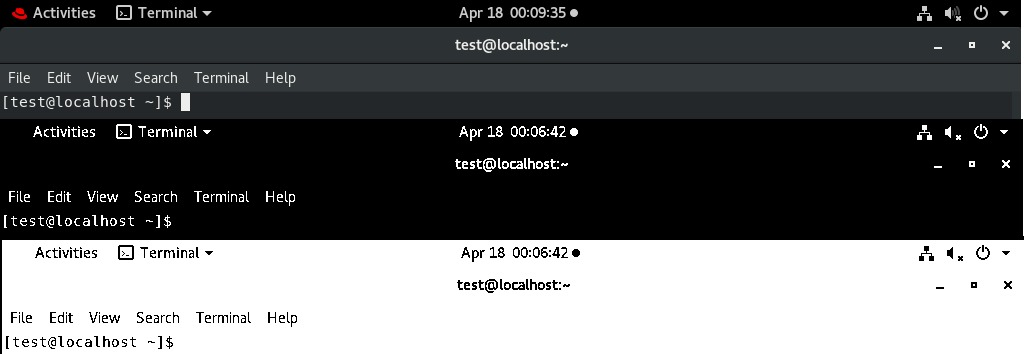
\includegraphics[width=1\textwidth,clip]{obrazky-figures/OCR_conversion.jpg}
	\caption{Steps of image preprocessing for Optical Character Recognition tool Tesseract, from the top: the original image, the binarized image, the inverted binarized image}
	\label{ocr_conversion}
\end{figure}

Listing \ref{OCR_text1} demonstrates the results obtained from the image, where the source image contains white text on a black background. The Tesseract's OCR engine manages to extract certain strings from the screen, although the results are not reliable and thus may lead to false-positive reports during the test execution.  

\begin{lstlisting}[caption={Text generated from the binarized image in Figure \ref{ocr_conversion}},label={OCR_text1}]
Pet) Terminal ~ EV ee muerre. Ty Pa) Ones
Peels ee?

Ca sa
[test@localhost ~]$ 
\end{lstlisting}

Listing \ref{OCR_text2} is showing the result of the character recognition when the image contains black text on a white background. When compared to Listings \ref{OCR_text1}, it proves an increase of the efficiency achieved with the implemented optimization. The result contains almost all strings shown on the screen with some random characters created as an attempt to read icons located in the right top corner of the window. The image conversions are achieved through methods from the \textit{OpenCV} library. 

\begin{lstlisting}[caption={Text generated from the inverted binarized image in Figure \ref{ocr_conversion}},label={OCR_text2}]
 Activities Terminal ~ Apr 18 00:22:36 AO Or
test@localhost:~ - 9 x

File Edit View Search Terminal Help
[test@localhost ~]$
\end{lstlisting}

Further experiments have shown additional issues with text formatting and recognition of certain letters. These facts led to another set of optimizations that were implemented to avoid false-positive test cases. A search for a string containing multiple words with white spaces might fail because the result might not contain all the white-spaces. Strings containing symbols …, -, \_, and — could be easily exchanged during the recognition. Those letters are not as important as letters representing the actual text. Therefore, a search for a match in the extracted text is performed twice. The first attempt tries to match the string with white spaces and full formatting. If that attempt fails, the second attempt breaks the string into words and tries to match every word separately. The second attempt is also followed by a warning message that the string was not matched in the original version.

The Tesseract has shown occasional difficulties with recognition of similarly looking letters. The most affected character was \textbf{I} exchanged for \textbf{1}, followed by \textbf{S} exchanged for \textbf{5}. Despite these occasional cases, the implementation works quite reliably both during the test generation process and the execution process. Nevertheless, the time consumed by taking screenshots during the generation process is significant. Therefore, the developed tool has the ability to disable the generation of the OCR steps during the generation of test cases through the command line parameter \texttt{-{}-disable-OCR}. If the generated test cases already contain steps performing OCR checks and are intended to be executed without them, the tests can be executed with the shell variable \texttt{OCR=False}. The defined variable will cause skipping of the OCR checks, although they will still be shown in the test logs as executed. This is caused by the limitation of the behave framework as it only allows to skip whole test scenarios. The test results executed with the variable will contain a warning message about skipped OCR steps.

\subsection{Implemented Steps}
The results obtained from experiments with the OCR were implemented to a single behave step. The step contains a string variable that should be found on the screen at a specific moment during the test execution. The process involves taking a screenshot via \texttt{gnome-screenshot} utility. It continues with image preprocessing and extraction of the text from two variants of images. Finally, an assertion is made to confirm the presence of the string on the screen. Listing \ref{ocr_test} contains a test case generated for \textit{Gedit} flatpak, in this case the OCR should confirm the presence of the \textit{Save} button on the screen. The introduced optimizations from the last section should help to avoid false-positive results. However, if the OCR fails to find the string on the screen, the error message printed to a log will contain all the extracted text. This should help the testers with easier identification of false-positives.

\begin{lstlisting}[language=Gherkin,caption={Test case demonstrating the OCR integration in test cases},label={ocr_test}]
    @18_Save
    Scenario: org.gnome.gedit: 18_Save
      * Start: "org.gnome.gedit" via command in session
      * State: "push button" "Save" "showing" is "True"
      * OCR: "Save" is shown on the screen
      * Action: "click" "Save" "push button"
      * State: "file chooser" "Save As" is shown
\end{lstlisting}


% implementation and testing, running in a VM and stuff

% An example of the generated test case scenario is available ....

\chapter{Testing and Results}
The result of the generation process is available in a folder structure containing generated test cases, configuration files, and scripts for execution in the CI environment. 

Generated test cases are located in the file named \texttt{generated.feature}. The file contains all the test cases divided into so-called scenarios. Each scenario has a unique name starting with character \texttt{@} that allows single test execution if required. All tests are executable by issuing a command \texttt{behave} in the generated project folder. The tests are also respecting the cleanup commands which are set in \texttt{apps.yaml}. The cleanup is always executed after the finish of the test, regardless of the result of the executed tests. Execution of \texttt{behave} either prints steps from a test scenario to standard output or can generate an HTML log. This log format is more suitable for examination of the results executed in the CI environment accessible through the web interface. 

Thanks to the setup done by the \textit{qecore} library, the \textit{behave} reports contain embedded logs, videos from the test runs, and a screenshot generated in a moment, when the test case fails. The next several sections describe the testing performed on several applications and the evaluation of the achieved results. The section starts with a short description of an application, followed by a result achieved by the proposed test generation tool.  

\section{Model/Event Coverage}
Test coverage can be measured in several ways. One option is to measure the amount of nodes and events covered by tests. The model is measured as the amount of the nodes involved in the test cases from the overall number of nodes in the model. It is expected that this coverage will always cover 100\% of the nodes. However, with applications that contain richer GUI, some of the nodes might be hidden or the generator will not be able to derive the sequence that will be able to access those nodes. This especially applies to cases when the generator will be used on a new application that contains some special layout or the action on the given node could not be executed for unknown reasons. The generator skips the whole test case, generates an error message, and proceeds to the next test case. 

Nodes that are not covered by tests, along with test sequences that are involved, are printed in a report after the test generator finishes.  The nodes or test sequences reported as failed must be evaluated manually with several possible outcomes:
\begin{enumerate}
    \item a bug in the tested application
    \item a bug in the accessibility (e.g. incorrectly reported coordinates)
    \item an imperfection/bug in the test generator
    \item the tested application is affected by the previous test case (change in the settings/layout), an additional cleanup must be added to \texttt{apps.yaml}
\end{enumerate}
The report not only serves as a feedback from the generator about potential issues but it also measures the event coverage. The event coverage measures the number of actions executed on the model and it is a common technique used in GUI testing\cite{NguyenBao2014Gait}.
Nevertheless, this approach also has a disadvantage. The event coverage report contains only events reported by the accessibility, other events like drag and drop, keyboard shortcuts and mouse scrolling are not included.

\section{Code Coverage}
Another possibility is to use a tool \verb|gcov|, which is a standard part of the GNU development tools. The purpose of the tool is Code Coverage Analysis and it was designed to find dead or unexecuted code. Code coverage analysis can be characterized by the following steps: 
\begin{enumerate}
  \item Find the areas of a program not exercised by the test suite.
  \item Create additional test cases to exercise the dead code, thereby increasing code coverage.
  \item Determine a quantitative measure of code coverage, which is an indirect measure of quality.
\end{enumerate}

To obtain a measurement of the code coverage, it's required to compile the application with \verb|gcc|/\verb|g++| and two extra parameters \verb|-fprofile-arcs| and \verb|-ftestcoverage|. Running the compiled binary with a \verb|gcov| tool will yield a percentage of the executed code located in source files. Measurements can be obtained for any software written in C/C++.\cite{gcov} 

To obtain measurements, tests must be executed with the custom binary, compiled with the mentioned parameters. Once the custom binary is executed, files with extensions \texttt{.gcda} and \texttt{.gcno} should appear in the directory where the binary is located. Measurements are aggregated throughout the test execution and the code coverage is reported to the special files with mentioned extensions. Then, the \texttt{lcov} tool is used to aggregate the measurements and generate a report in two steps (Code Listing \ref{lcov_report}). The first command takes the\texttt{.gcda} and \texttt{.gcno} files and generates \texttt{.info} file with coverage info. The second command takes the \texttt{info} file and generates a detailed HTML report. The report contains every source file (\texttt{.c} file) along with the percentage of covered functions and lines.

\begin{lstlisting}[language=Gherkin,caption={Shell commands used to generate an HTML report with \texttt{lcov} tool},label={lcov_report}]
    lcov -c -d . -o app.info
    genhtml -o lcov_report -s --legend app.info --ignore-errors
\end{lstlisting}

According to the GTK website\footnote{\url{https://www.gtk.org/}}, the framework supports JavaScript, Python, Rust, Vala, C, and Perl. The \verb|gcov| method of measuring the test coverage is only possible for C and Vala.    
%test coverage, node coverage, action coverage
\section{Test Environment}
All performed testing was done on virtual machines preloaded with distributions \textit{Red Hat Enterprise Linux 8.2/8.3} and \textit{Fedora 31/32}. The execution of the test generator on production workstations should be avoided as the performed actions may potentially lead to alteration of the system or data loss.  This also applies to the generated test cases. 

\section{GNOME Terminal Tests}
% code coverage, explanation of achieved coverage
GNOME Terminal is one of the most important applications from the GNOME application stack. It is also known as \textit{Terminal} and it serves as a terminal emulator for accessing a UNIX shell environment. The application can be used to run programs available on the system\footnote{\url{https://help.gnome.org/users/gnome-terminal/stable/introduction.html.en}}. Compared to the majority of GNOME applications, \textit{Terminal} does not contain as many UI elements (Figure \ref{terminal-gui}). Therefore, it was used for the initial development of the test generator. Shortly after the first proof of concept was tested, the list of applications was extended to \textit{LibreOffice Start Center} and \textit{Gedit}. 

\begin{figure}[H]
	\centering
	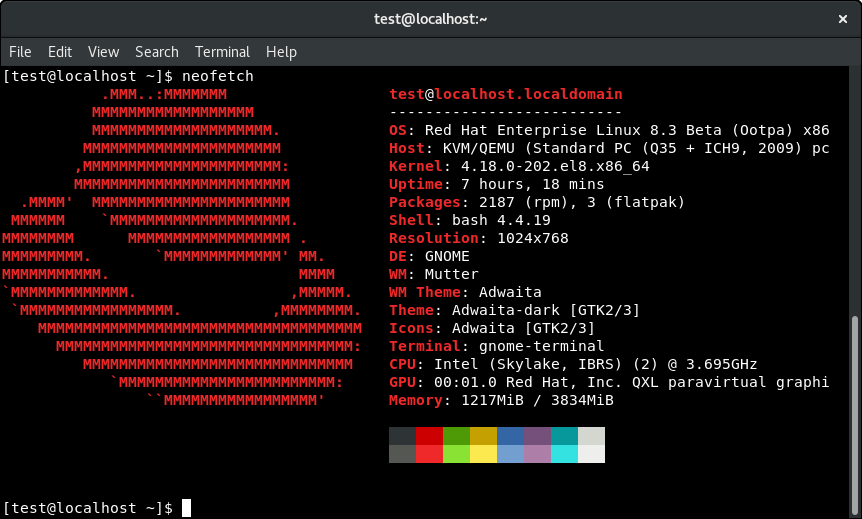
\includegraphics[width=0.75\textwidth,clip]{obrazky-figures/gnome-terminal-ui.png}
	\caption{GNOME Terminal application UI}
	\label{terminal-gui}
\end{figure}

\subsection{Setup and Cleanup}
Greater part of test cases is performing some changes of settings either via \textit{Preferences} dialog or through menus located at the top of the window. Preferences can change various aspects of the application, including encoding, layout of widgets, and color schemes. Those changes need to be set back to default values to make sure that test cases won't affect subsequent test cases. In \textit{Terminal}, this is achieved through 2 cleanup commands executed between applied test sequences (Code Listing \ref{gnome-terminal-cleanup}). Testing was performed with rpm package \texttt{gnome-terminal-3.28.3-1.el8.x86\_64}, Red Hat Enterprise Linux 8.3.

\begin{lstlisting}[caption={Final test generator report},label={gnome-terminal-cleanup}]
    dconf reset /org/gtk/Settings/Debug/enable-inspector-keybinding
    dconf reset -f /org/gnome/terminal/legacy/
\end{lstlisting}

\subsection{Test Generation and Results}

Listing \ref{gnome-terminal-report} contains the final report and summarizes the testing performed on \textit{Terminal}. The developed test generator was able to generate 485 test cases while covering the 1701 events in the application. Tests are covering menus, several smaller dialogs, and a \textit{Preferences} window.

\begin{lstlisting}[caption={Final test generator report},label={gnome-terminal-report}]
    Event Coverage Report:
        Covered Events: 1700/1702
        Number of covered Nodes: 516
        Number of Generated Test Cases: 485 
        Nodes without the coverage:
            Edit:menu:click => Preferences:menu item:click => :list item: 
                => Menu:toggle button:click
            Help:menu:click => About:menu item:click => :link:Click
    No errors found!
    Generation time: 1:53:52.676497s
\end{lstlisting}

Generated test cases covered 34.2\% lines of source code and executed 42\% of functions (Figure \ref{gnome-terminal-coverage}). As described in the report, the coverage resides in the low category. After looking to the report in detail and reading the comments in source code, the analysis has shown that several parts of the GUI are not executed by the tests. It has revealed functions that are handling shortcuts that are not covered in the test cases. It is also expected that a large portion of code is related to non-GUI operations which are not covered in tests at all.

\begin{figure}[H]
	\centering
	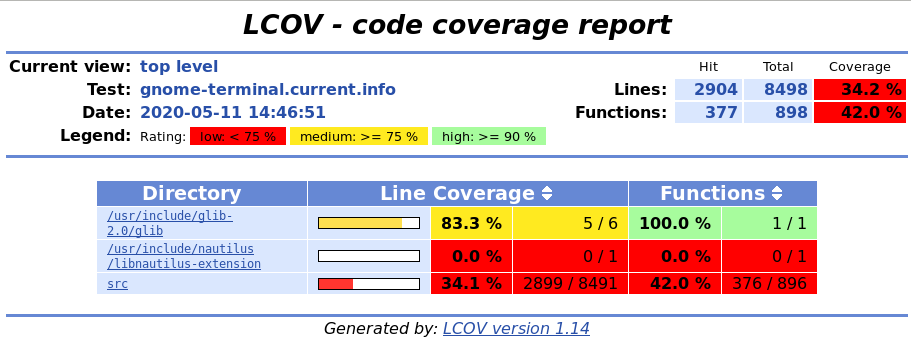
\includegraphics[width=0.8\textwidth,clip]{obrazky-figures/gnome-termina-coverage.png}
	\caption{Achieved code coverage report for GNOME Terminal}
	\label{gnome-terminal-coverage}
\end{figure}

\textit{Terminal} also offered a good demonstration of how nodes are expanded during the test generation. Initially, the generator scans the tree for the available nodes and builds a model from 104 available nodes (widgets) and derives 96 test sequences (Figure \ref{gnome-terminal-graph1}). The Generator proceeds with the application of sequences and continuously expands the model to the final amount of 516 nodes and 485 derived test cases (Figure \ref{gnome-terminal-graph2}).

\begin{figure}[H]
	\centering
	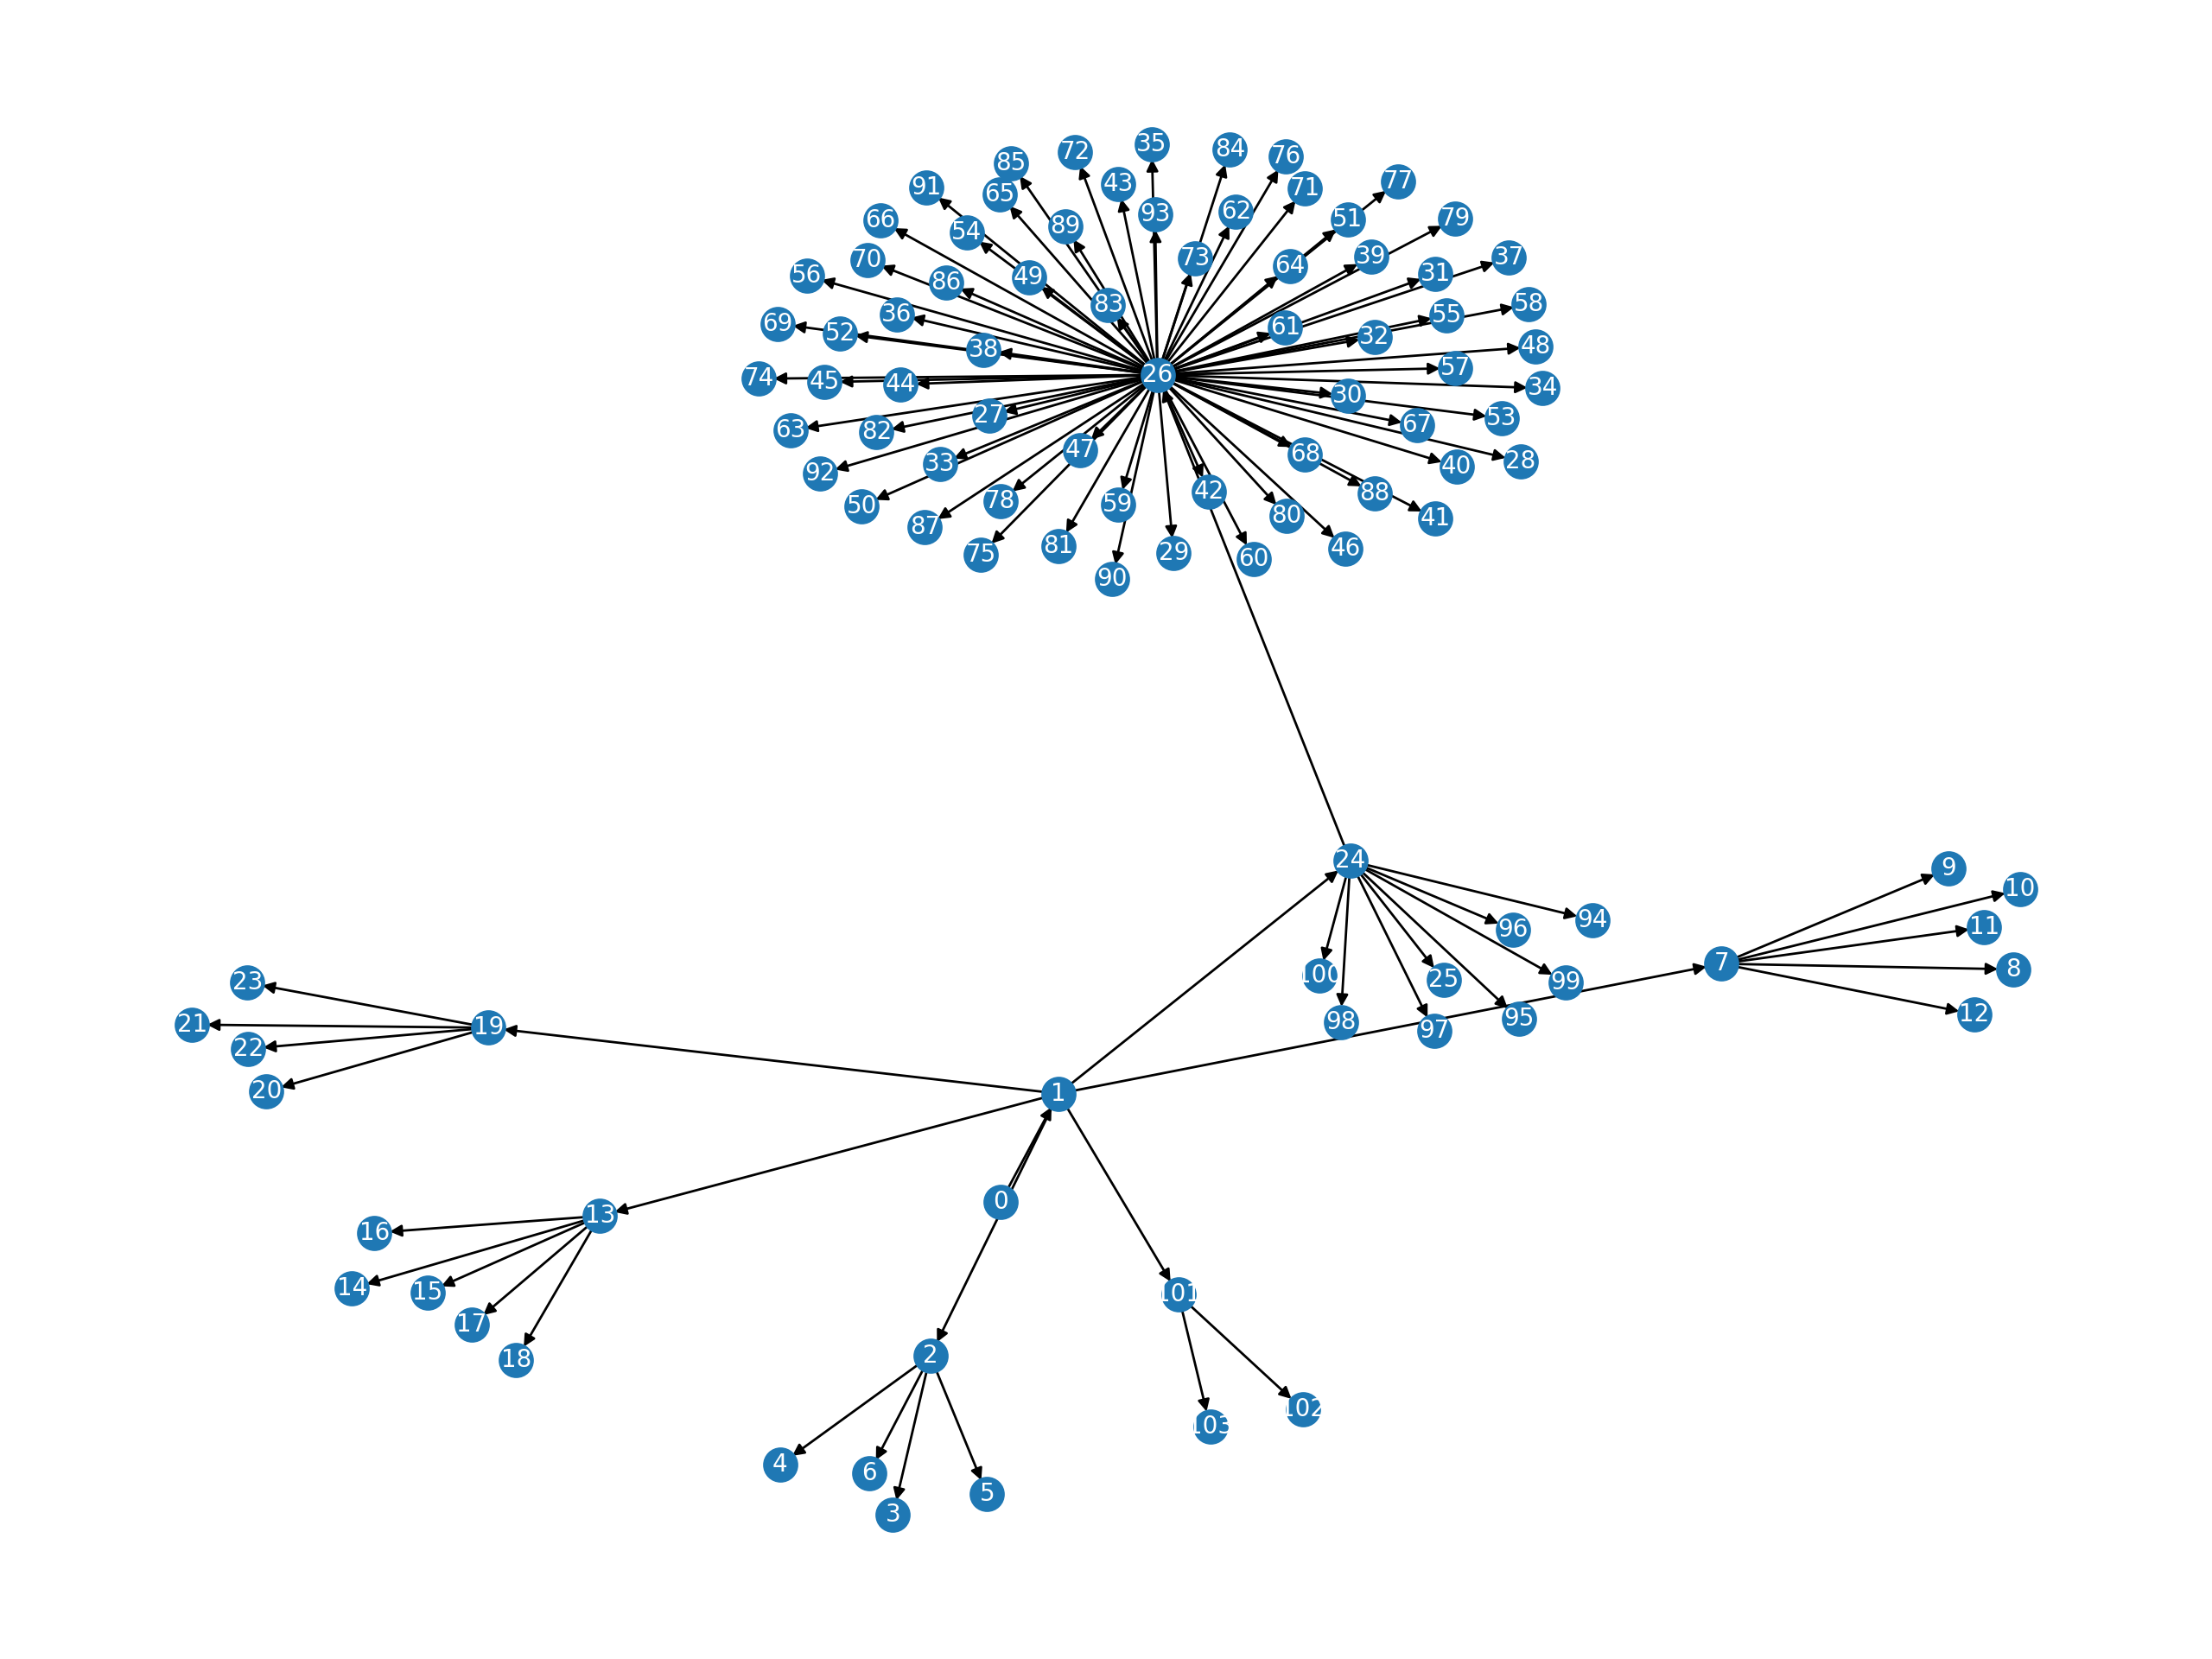
\includegraphics[width=0.85\textwidth,clip]{obrazky-figures/gnome-terminal_n_start.png}
	\caption{Initial event flow graph for GNOME Terminal}
	\label{gnome-terminal-graph1}
\end{figure}

\begin{figure}[H]
	\centering
	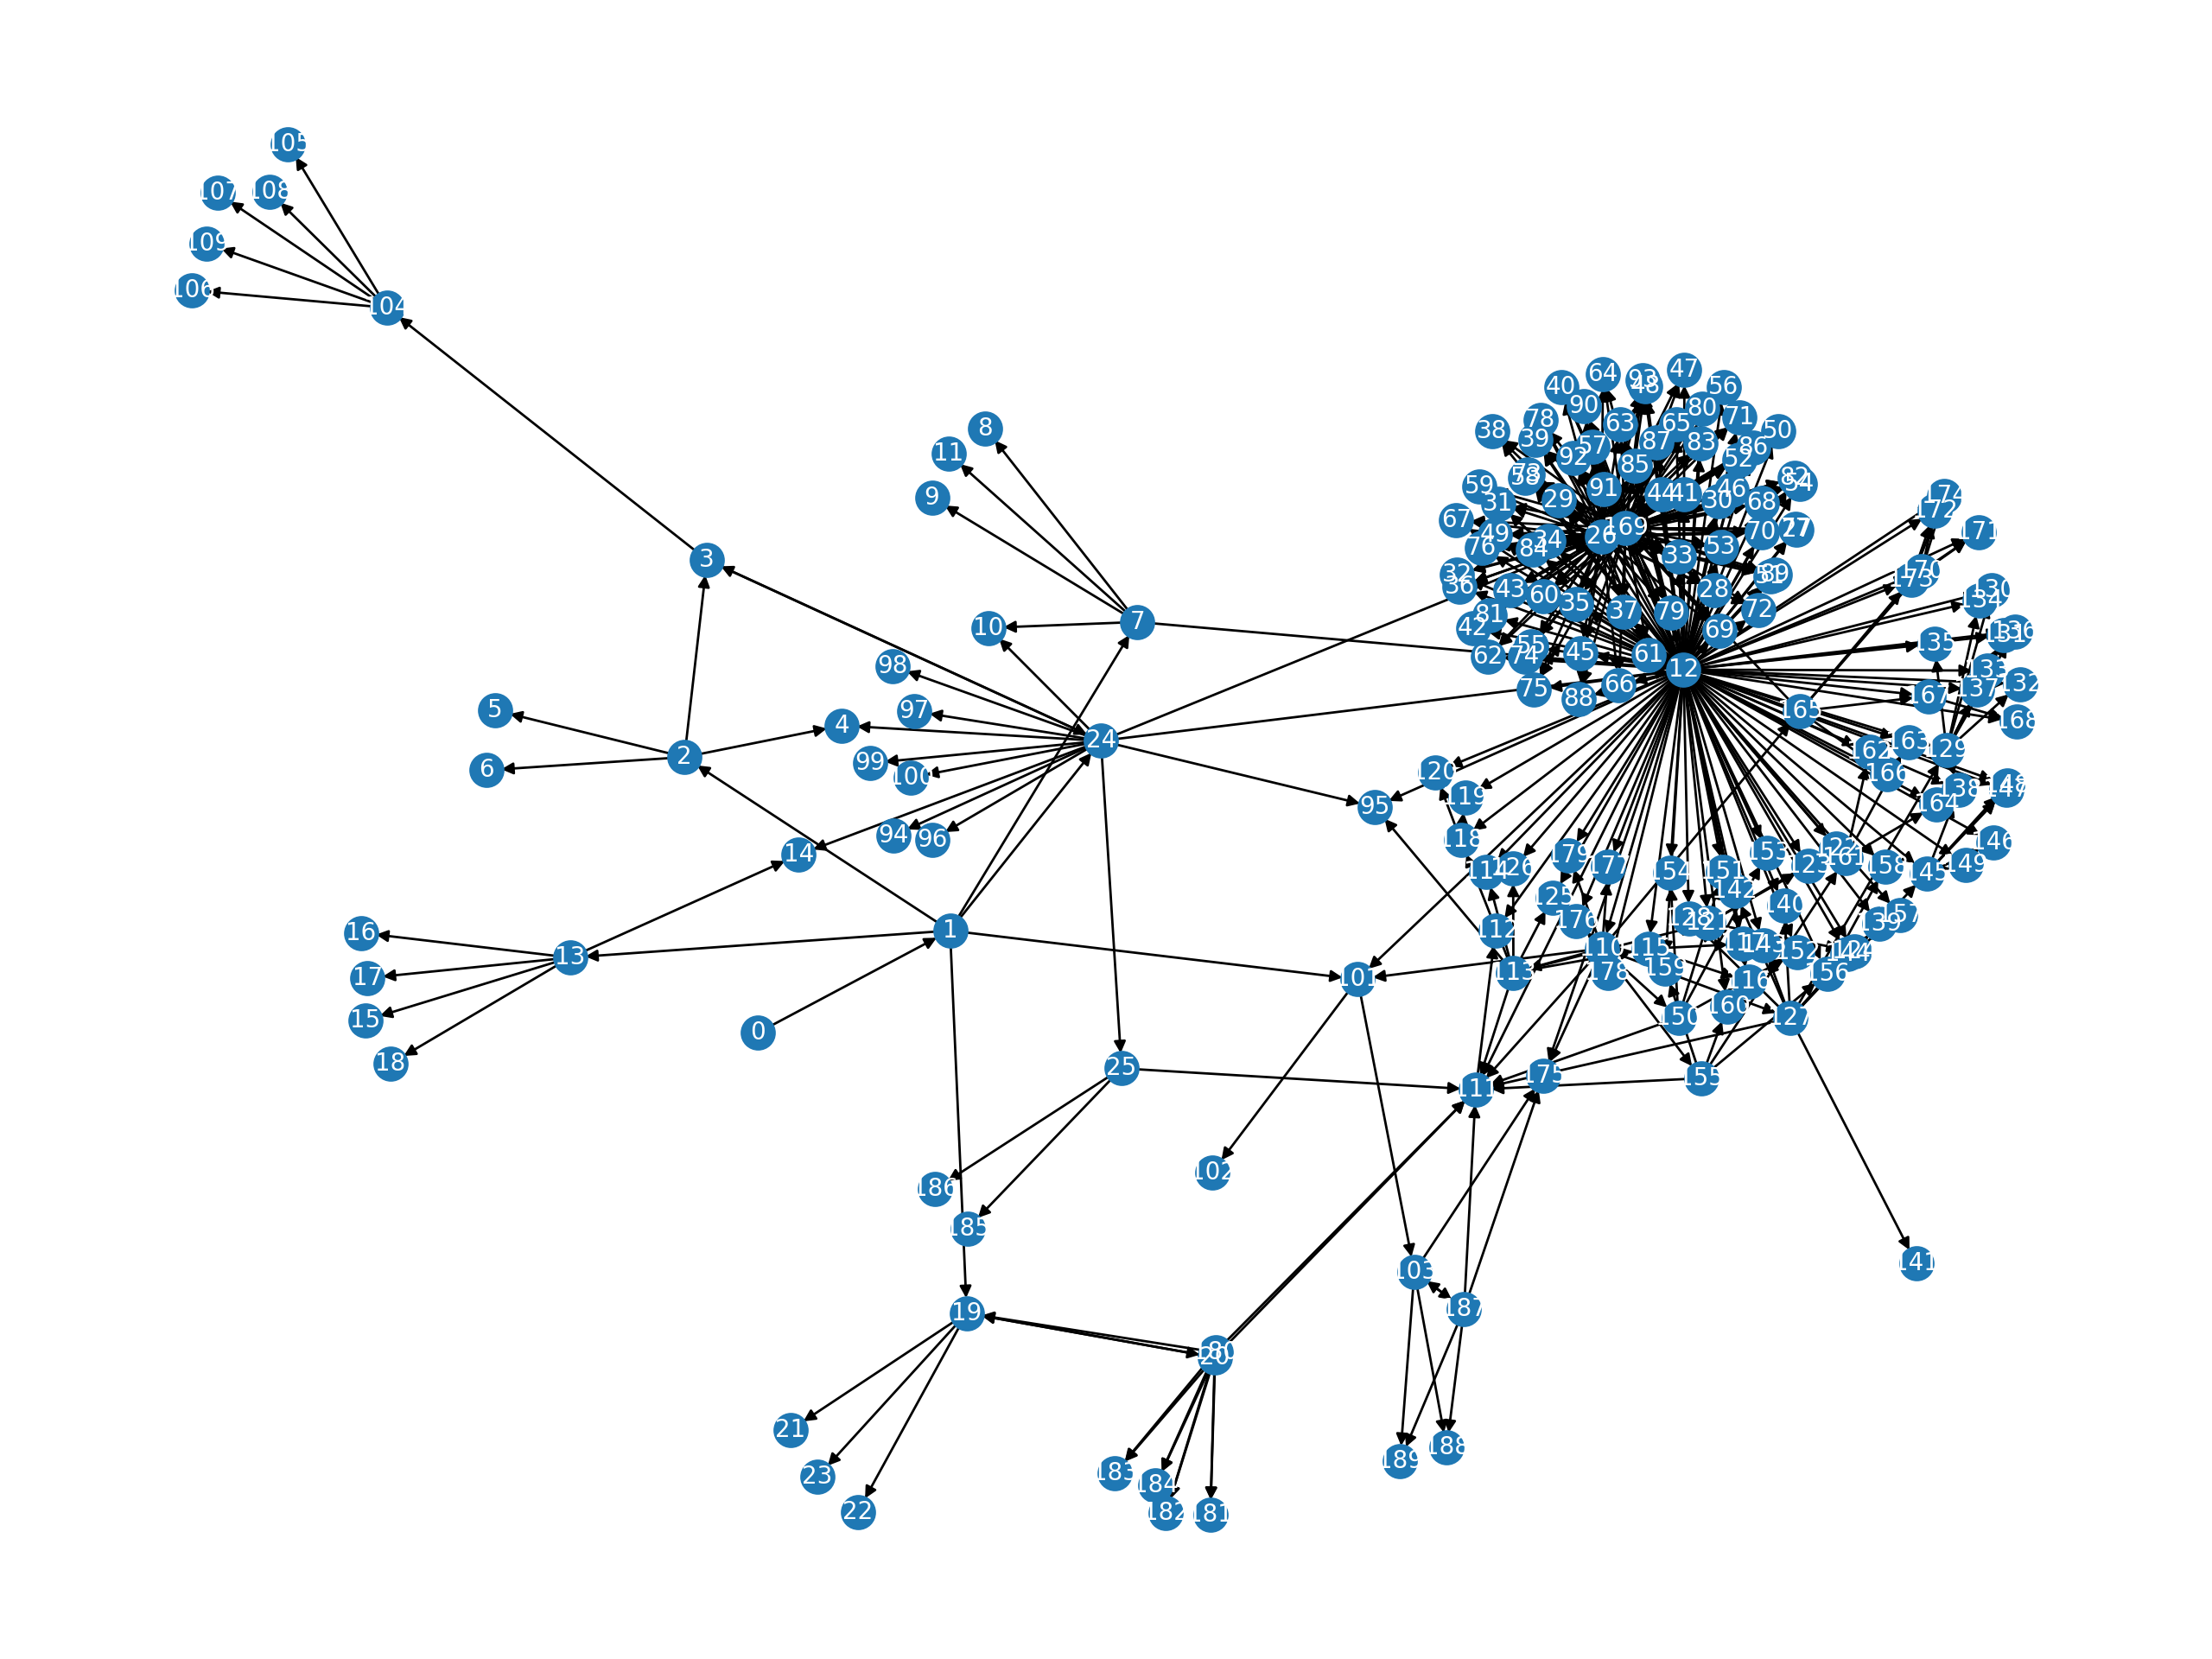
\includegraphics[width=0.85\textwidth,clip]{obrazky-figures/gnome-terminal_n_final.png}
	\caption{Expanded event flow graph for GNOME Terminal}
	\label{gnome-terminal-graph2}
\end{figure}

\section{GNOME Help}
GNOME Help (or yelp) is a help viewer for GNOME\footnote{\url{https://wiki.gnome.org/Apps/Yelp}}. The application natively renders documents in various formats including HTML documents. The UI is filled with links to navigate between documents.

\begin{figure}[H]
	\centering
	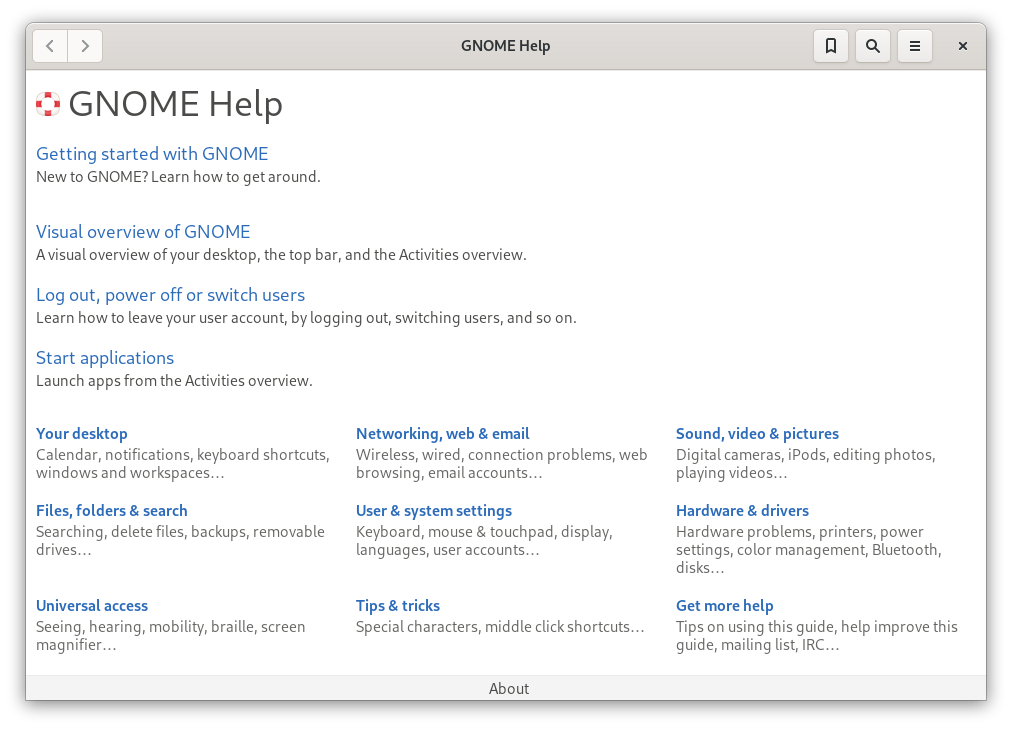
\includegraphics[width=0.75\textwidth,clip]{obrazky-figures/yelp-ui.png}
	\caption{GNOME Help (Yelp) application UI}
	\label{yelp_ui}
\end{figure}

\subsection{Test Generation and Results}

Listing \ref{yelp-report} contains the final report and summarizes the testing performed on \textit{GNOME Help}. The developed test generator was able to generate 2415 test cases while covering the 4690 events in the application. The application did not require any individual setup, testing was performed with rpm package \texttt{yelp-3.28.1-3.el8.x86\_64}.

\begin{lstlisting}[caption={Final test generator report},label={yelp-report}]
    Event Coverage Report:
    Covered Events: 4690/4696
    Number of covered Nodes: 2415
    Number of Generated Test Cases: 2412
    Nodes without the coverage:
    GNOME Help:frame: => Digital cameras:link:jump 
                => More Information:heading:Click
    ...
    GNOME Help:frame: => playing videos:link:jump
                => More Information:heading:Click 
    Generation time: 4:57:13.370368s
\end{lstlisting}

The 6 missing events are reported by the test generator along with test sequences in which they are included. Those sequences are generated because the accessibility reports and unknown action that can be performed on nodes with role name \texttt{heading}. The test generator cannot perform the action, therefore it tries to replace the associated action with the default one - Click. Since the execution of the event failed, nodes were left without event coverage. This can be categorized as another imperfection in accessibility and can be solved by adding the role name of the node to the list of actionless nodes \texttt{rolenames.py}. However, blacklisting the role name \texttt{heading} caused a disappearance of \textasciitilde600 test cases. This implies that only those 6 reported nodes were mislabeled and nodes with the role name \texttt{heading} should not be blacklisted.  

The second part of the report is dedicated to captured error messages. Overall, there were 42 warnings about occurrences of error messages during the test generation along with reproducers. The examination of the reproducers has revealed a bug\footnote{\url{https://bugzilla.redhat.com/show_bug.cgi?id=1837978}} in Firefox. 

Initially, the generator started with a group of 78 nodes (Figure \ref{yelp_start}) that was expanded to the final number of 2415 nodes (Figure \ref{yelp_end}). When compared to manual testing, the effort required to achieve this would be very tedious and time-consuming. 


\begin{figure}[H]
	\centering
	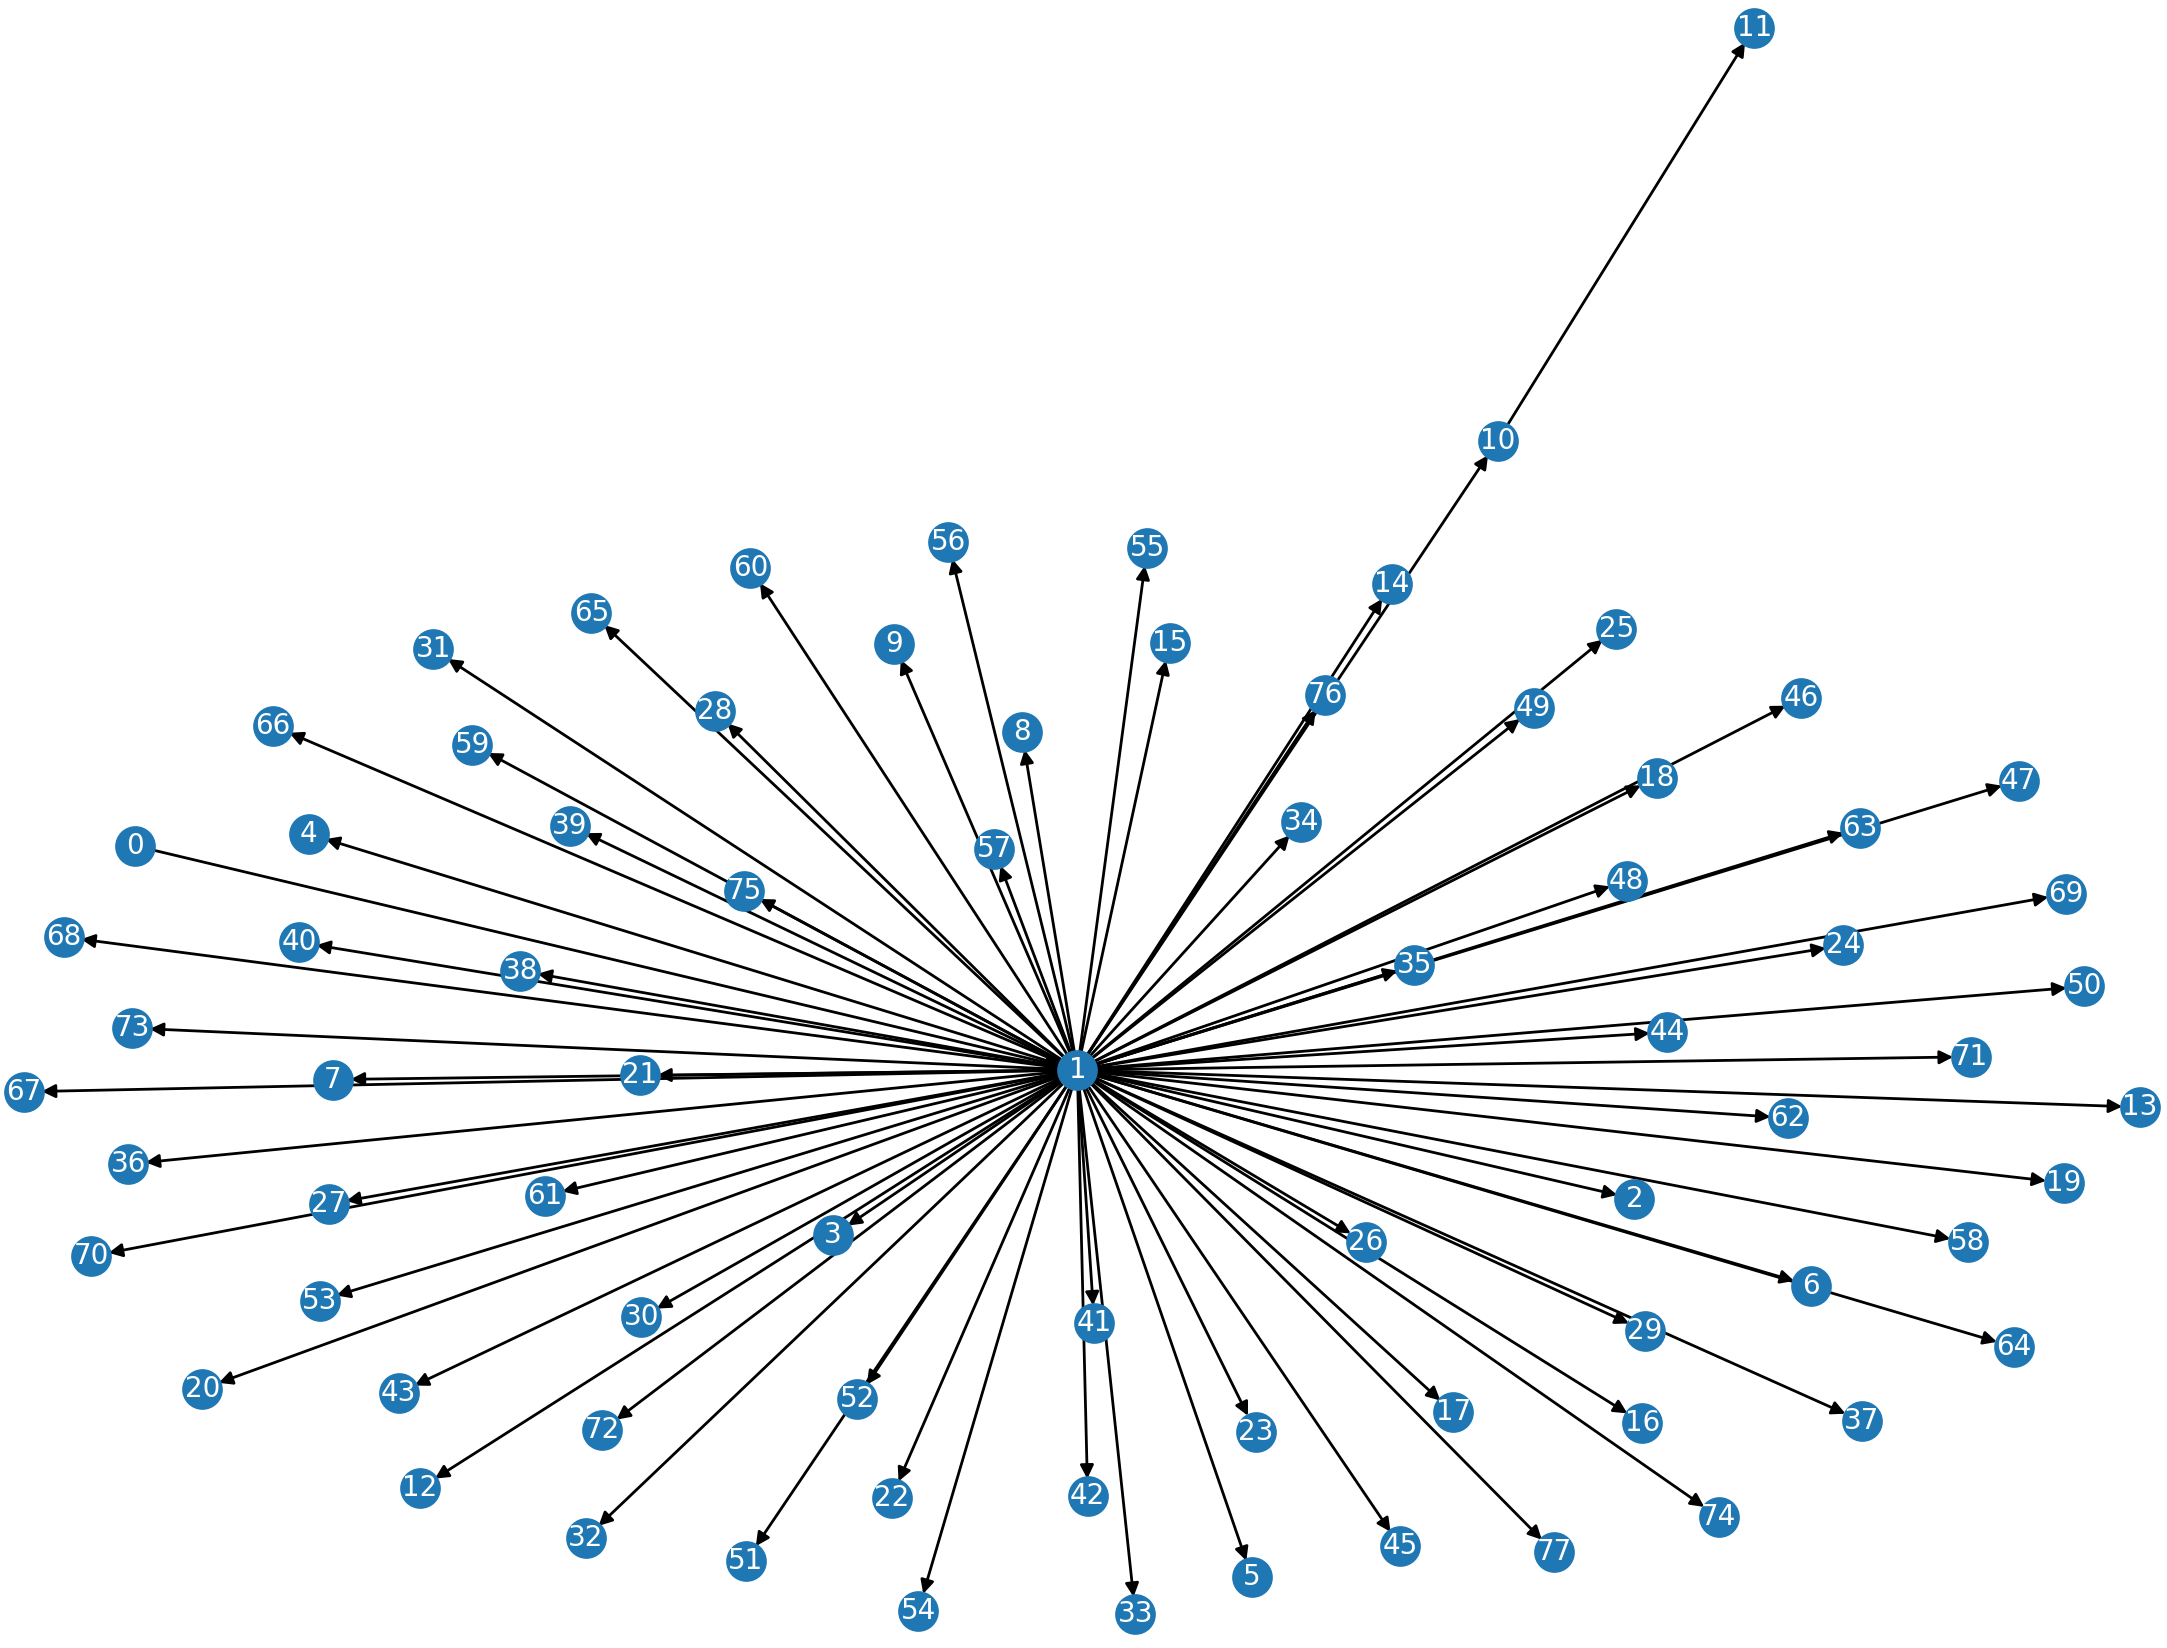
\includegraphics[width=1\textwidth,clip]{obrazky-figures/yelp_n_start.png}
	\caption{Initial event flow graph of test sequences for GNOME Help}
	\label{yelp_start}
\end{figure}

\begin{figure}[H]
	\centering
	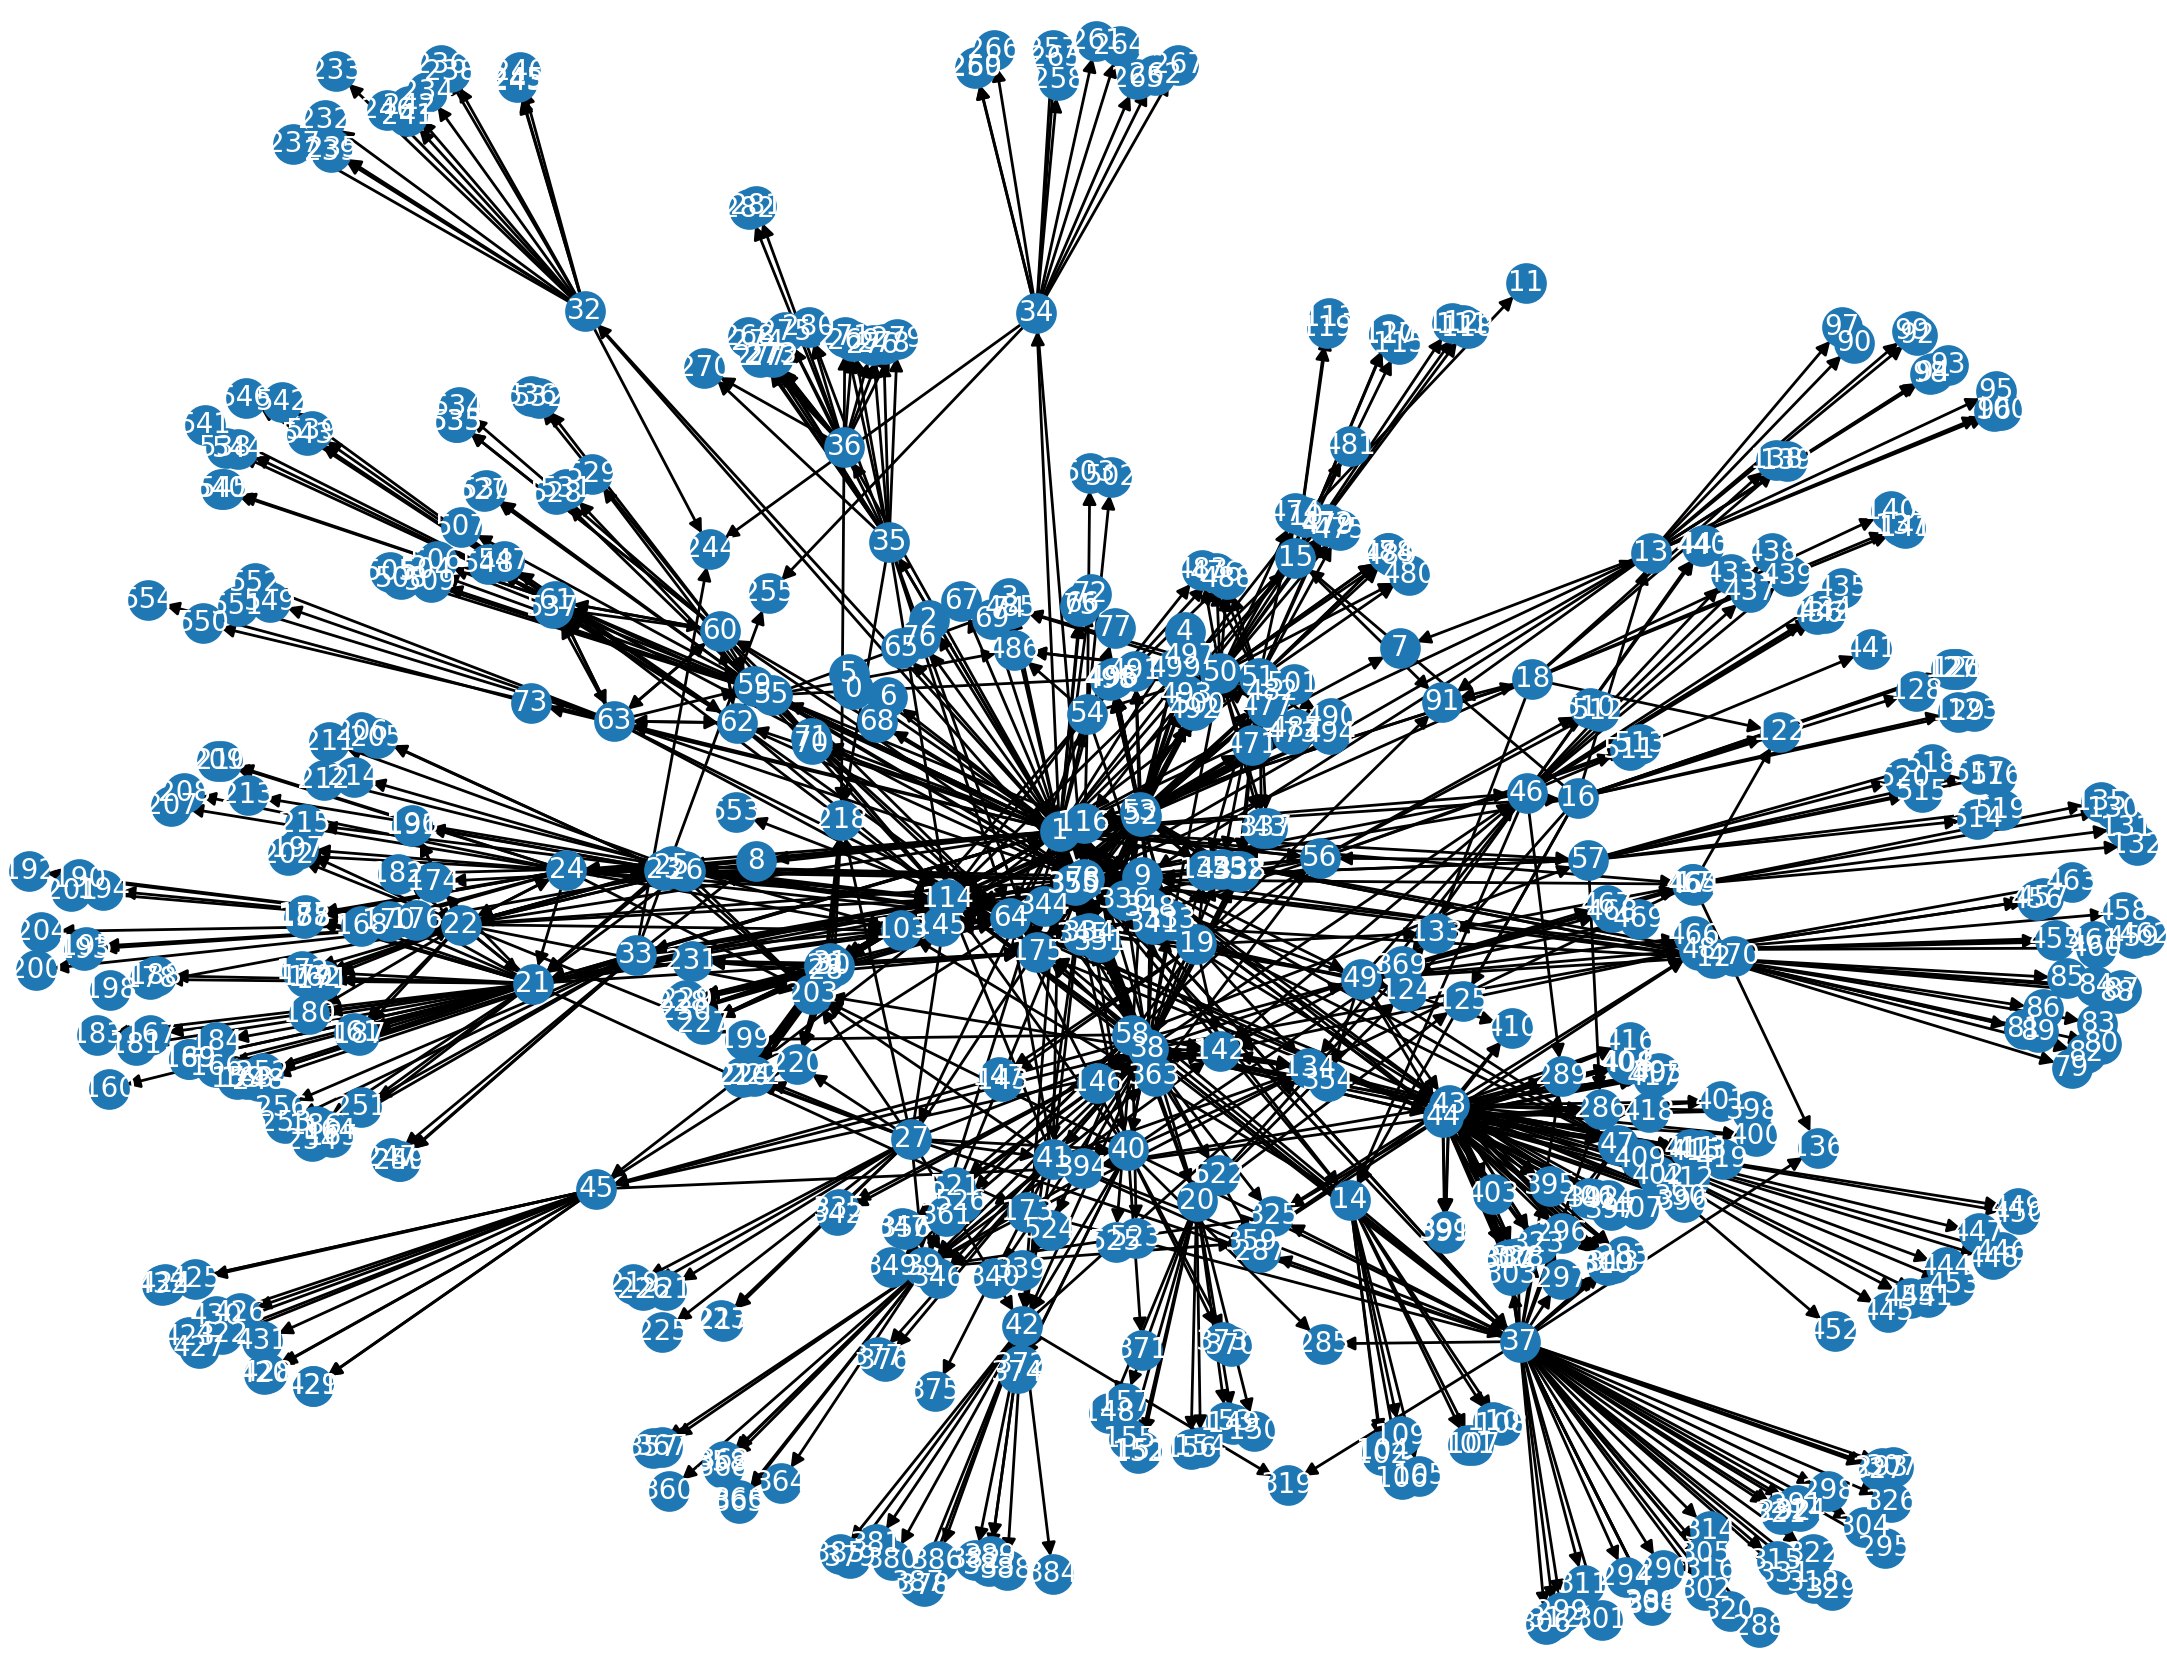
\includegraphics[width=0.85\textwidth,clip]{obrazky-figures/yelp_n_final.png}
	\caption{Expanded event flow graph of test sequences for GNOME Help}
	\label{yelp_end}
\end{figure}

% \section{Gedit (flatpak)}
\section{LibreOffice StartCenter}

LibreOffice StartCenter (\ref{libreoffice-gui}) is a document management application, it connects 7 other applications from the document suite. Each application can open and edit different for format of documents\footnote{\url{https://help.libreoffice.org/3.3/Common/Start_Center}}. LibreOffice is not a part of the GNOME application stack although it is being shipped as a default document suite in a lot of Linux distributions and has the accessibility support.

\begin{figure}[H]
	\centering
	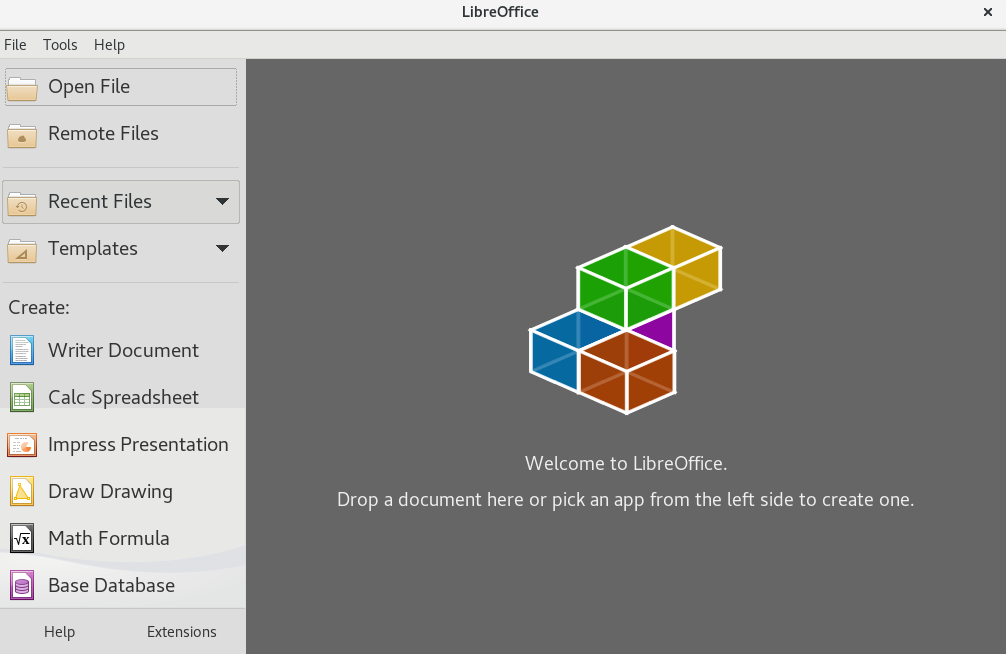
\includegraphics[width=0.85\textwidth,clip]{obrazky-figures/libreoffice_GUI.png}
	\caption{LibreOffice StartCenter}
	\label{libreoffice-gui}
\end{figure}


\subsection{Required Implementation Changes and Limitations}
Several complications required application-specific changes to be added in the implementation of the test generator. 

Tests are executing all applications from the LibreOffice Suite. LibreOffice Calc is a spreadsheet editor that contains theoretically an infinite number of cells that could be edited. Therefore, the application cannot be recursively explored for new nodes. A recursive search causes that the application will generate new cells until the RAM on a virtual machine is depleted. The virtual machine is unresponsive and refuse to execute commands through a remote shell. Therefore, the implementation of the test generator was altered to avoid the execution of a recursive search on Libreoffice Calc.

Another accessibility-related issue has started to occur when the test generation process reached certain types of dialogs (letter wizard, fax wizard, etc.). The behavior was quite similar to the previous issue, the test generator hanged on a recursive search query for a while and then failed with the error message shown in Listing \ref{error-message}.

\begin{lstlisting}[caption={The error that prevents the generator from node expansion},label={error-message}]
Failed to handle new nodes atspi_error: The application no longer exists (0)
\end{lstlisting}

 The investigation has shown the application spawns 2 windows, the first one is a previously mentioned dialog, the second one is a generic Libreoffice window that contains only a blank window with menus. The blank window is probably spawned because those wizard dialogs are not standalone applications, they belong to other applications from the LibreOffice suite. This claim is supported by the fact that the blank window only lasts as long as the dialog is opened. The blank window contains widgets but they are not available for interaction as the focus is only available for the dialog window in the front. Therefore, the blank window is an issue from the implementation perspective of the generator as it tries to perform node expansion on a window that never becomes available. Since the accessibility throws the mentioned error, it is handled as an exception and the generator continues without expansion of affected part of the application.

\subsection{Testing and Results}
LibreOffice test required some setup in the \texttt{apps.yaml} file. The application instance has to be started with a \texttt{-{}-norestore} parameter to avoid the restoration of unsaved documents from previous sessions. The user configurations files located in \texttt{\textasciitilde/.config/libreoffice/} are removed during the cleanup process. After previously discussed implementation changes, the generator has been able to perform the full run on the application and produce a test report that is partially shown in Code Listing \ref{yelp-report}.


\begin{lstlisting}[caption={Final test generator report for LibreOffice StartCenter},label={yelp-report}]
    Event Coverage Report:
    Covered Events: 7795/7853 (99.26%) 
    Number of covered Nodes: 2516
    Number of Generated Test Cases: 2315
    Nodes without the coverage:
    ...
    Generation time: 11:48:49.071478s
\end{lstlisting}

The report shows that the achieved event coverage was not as successful as with the previous components. The majority of the failed sequences contained nodes that have the action available, but they were not available for interaction at a given time. 

The report also contained several crashes. One of the crashes has been revealed quite early and was reported as a bug\footnote{\url{https://bugzilla.redhat.com/show_bug.cgi?id=1819798}}. Another group of crashes was caused by quite an interesting phenomenon. The test generator reported 6 crashes with steps to reproduce them. Manual examination of the reproducers as shown similar pattern in all crashed. Each crash by triggering an action on a button that was not available for interaction. The issue could not be reproduced from the user perspective, the event can only be sent through the accessibility. Nevertheless, this proves that the proposed solution can reveal this kind of flaws in software.

Despite the fact that node expansion during the generation process was affected by the discussed issues with the accessibilitty, the achieved results are presented in the Figure \ref{libreoffice-graph1} and \ref{libreoffice-graph2}.

LibreOffice documentation contains the guide\footnote{\url{https://wiki.documentfoundation.org/Development/Lcov}}  on how to obtain code coverage measurements written in the year 2013. However, I haven't been able to rebuild the whole suite with required flags. Therefore, I did not acquired code coverage measurements for this application.   


\begin{figure}[H]
	\centering
	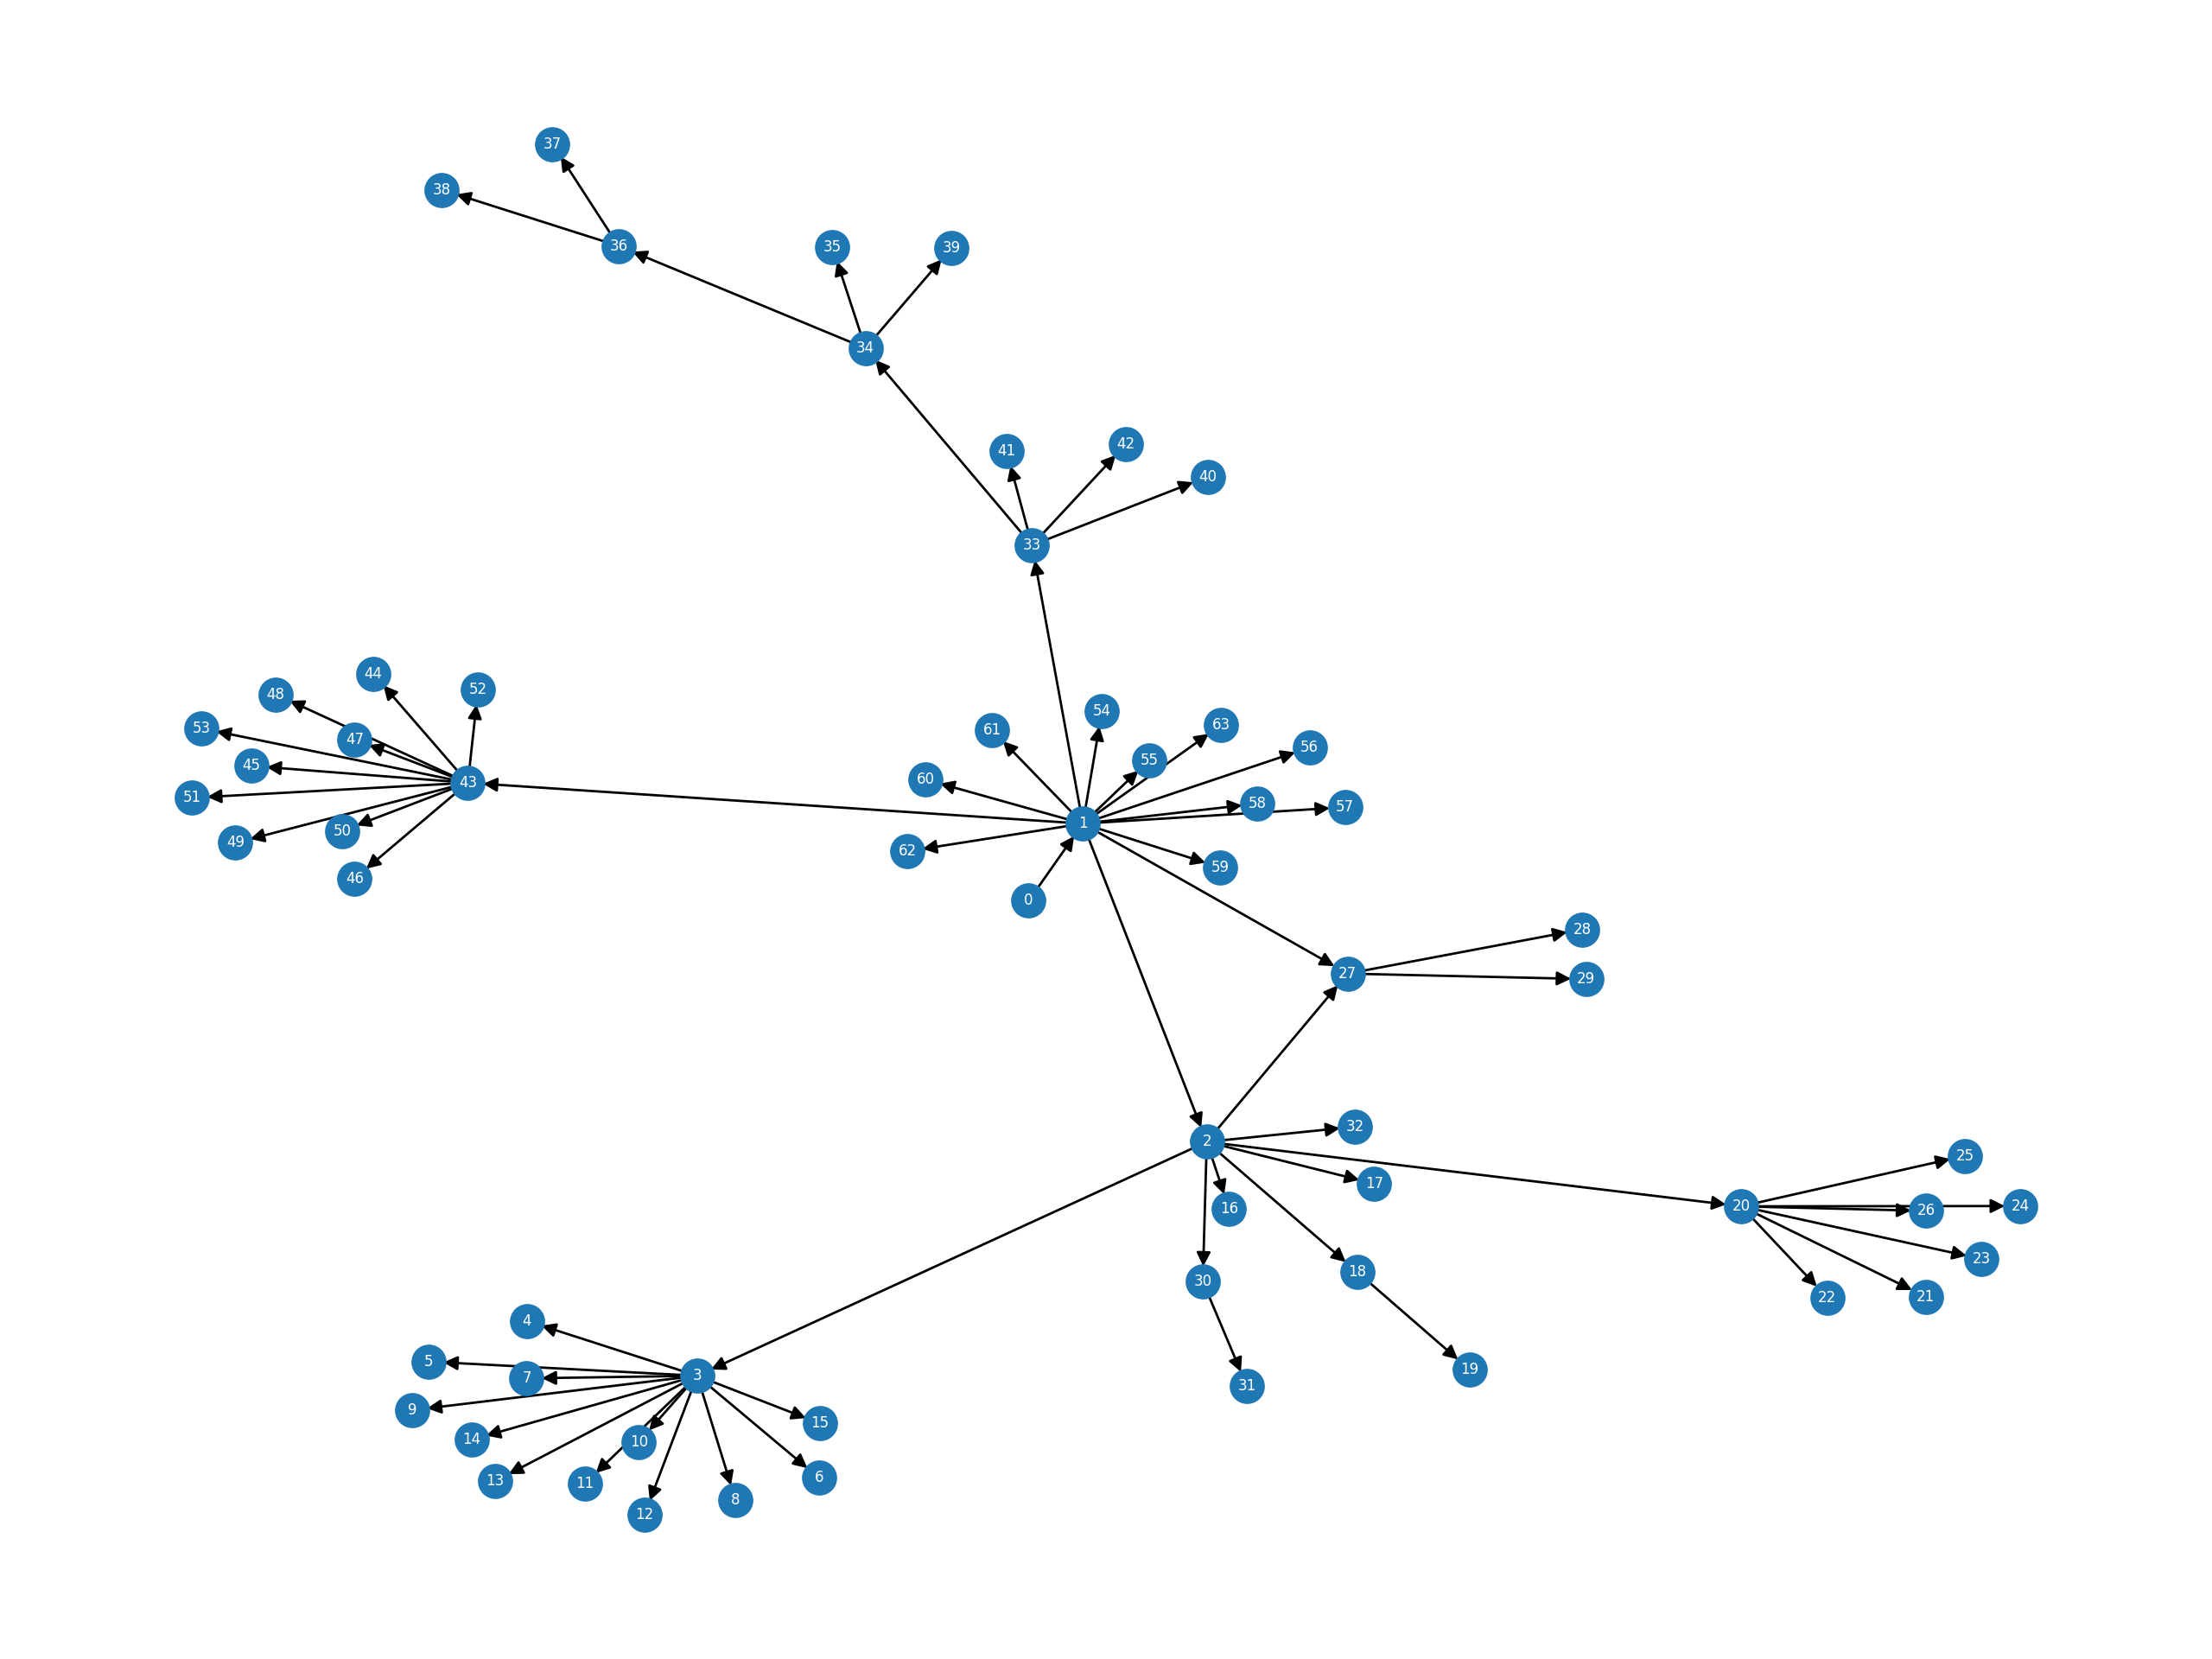
\includegraphics[width=0.85\textwidth,clip]{obrazky-figures/liibreoffice_n_start.png}
	\caption{Initial event flow graph after the start of LibreOffice StartCenter}
	\label{libreoffice-graph1}
\end{figure}

\begin{figure}[H]
	\centering
	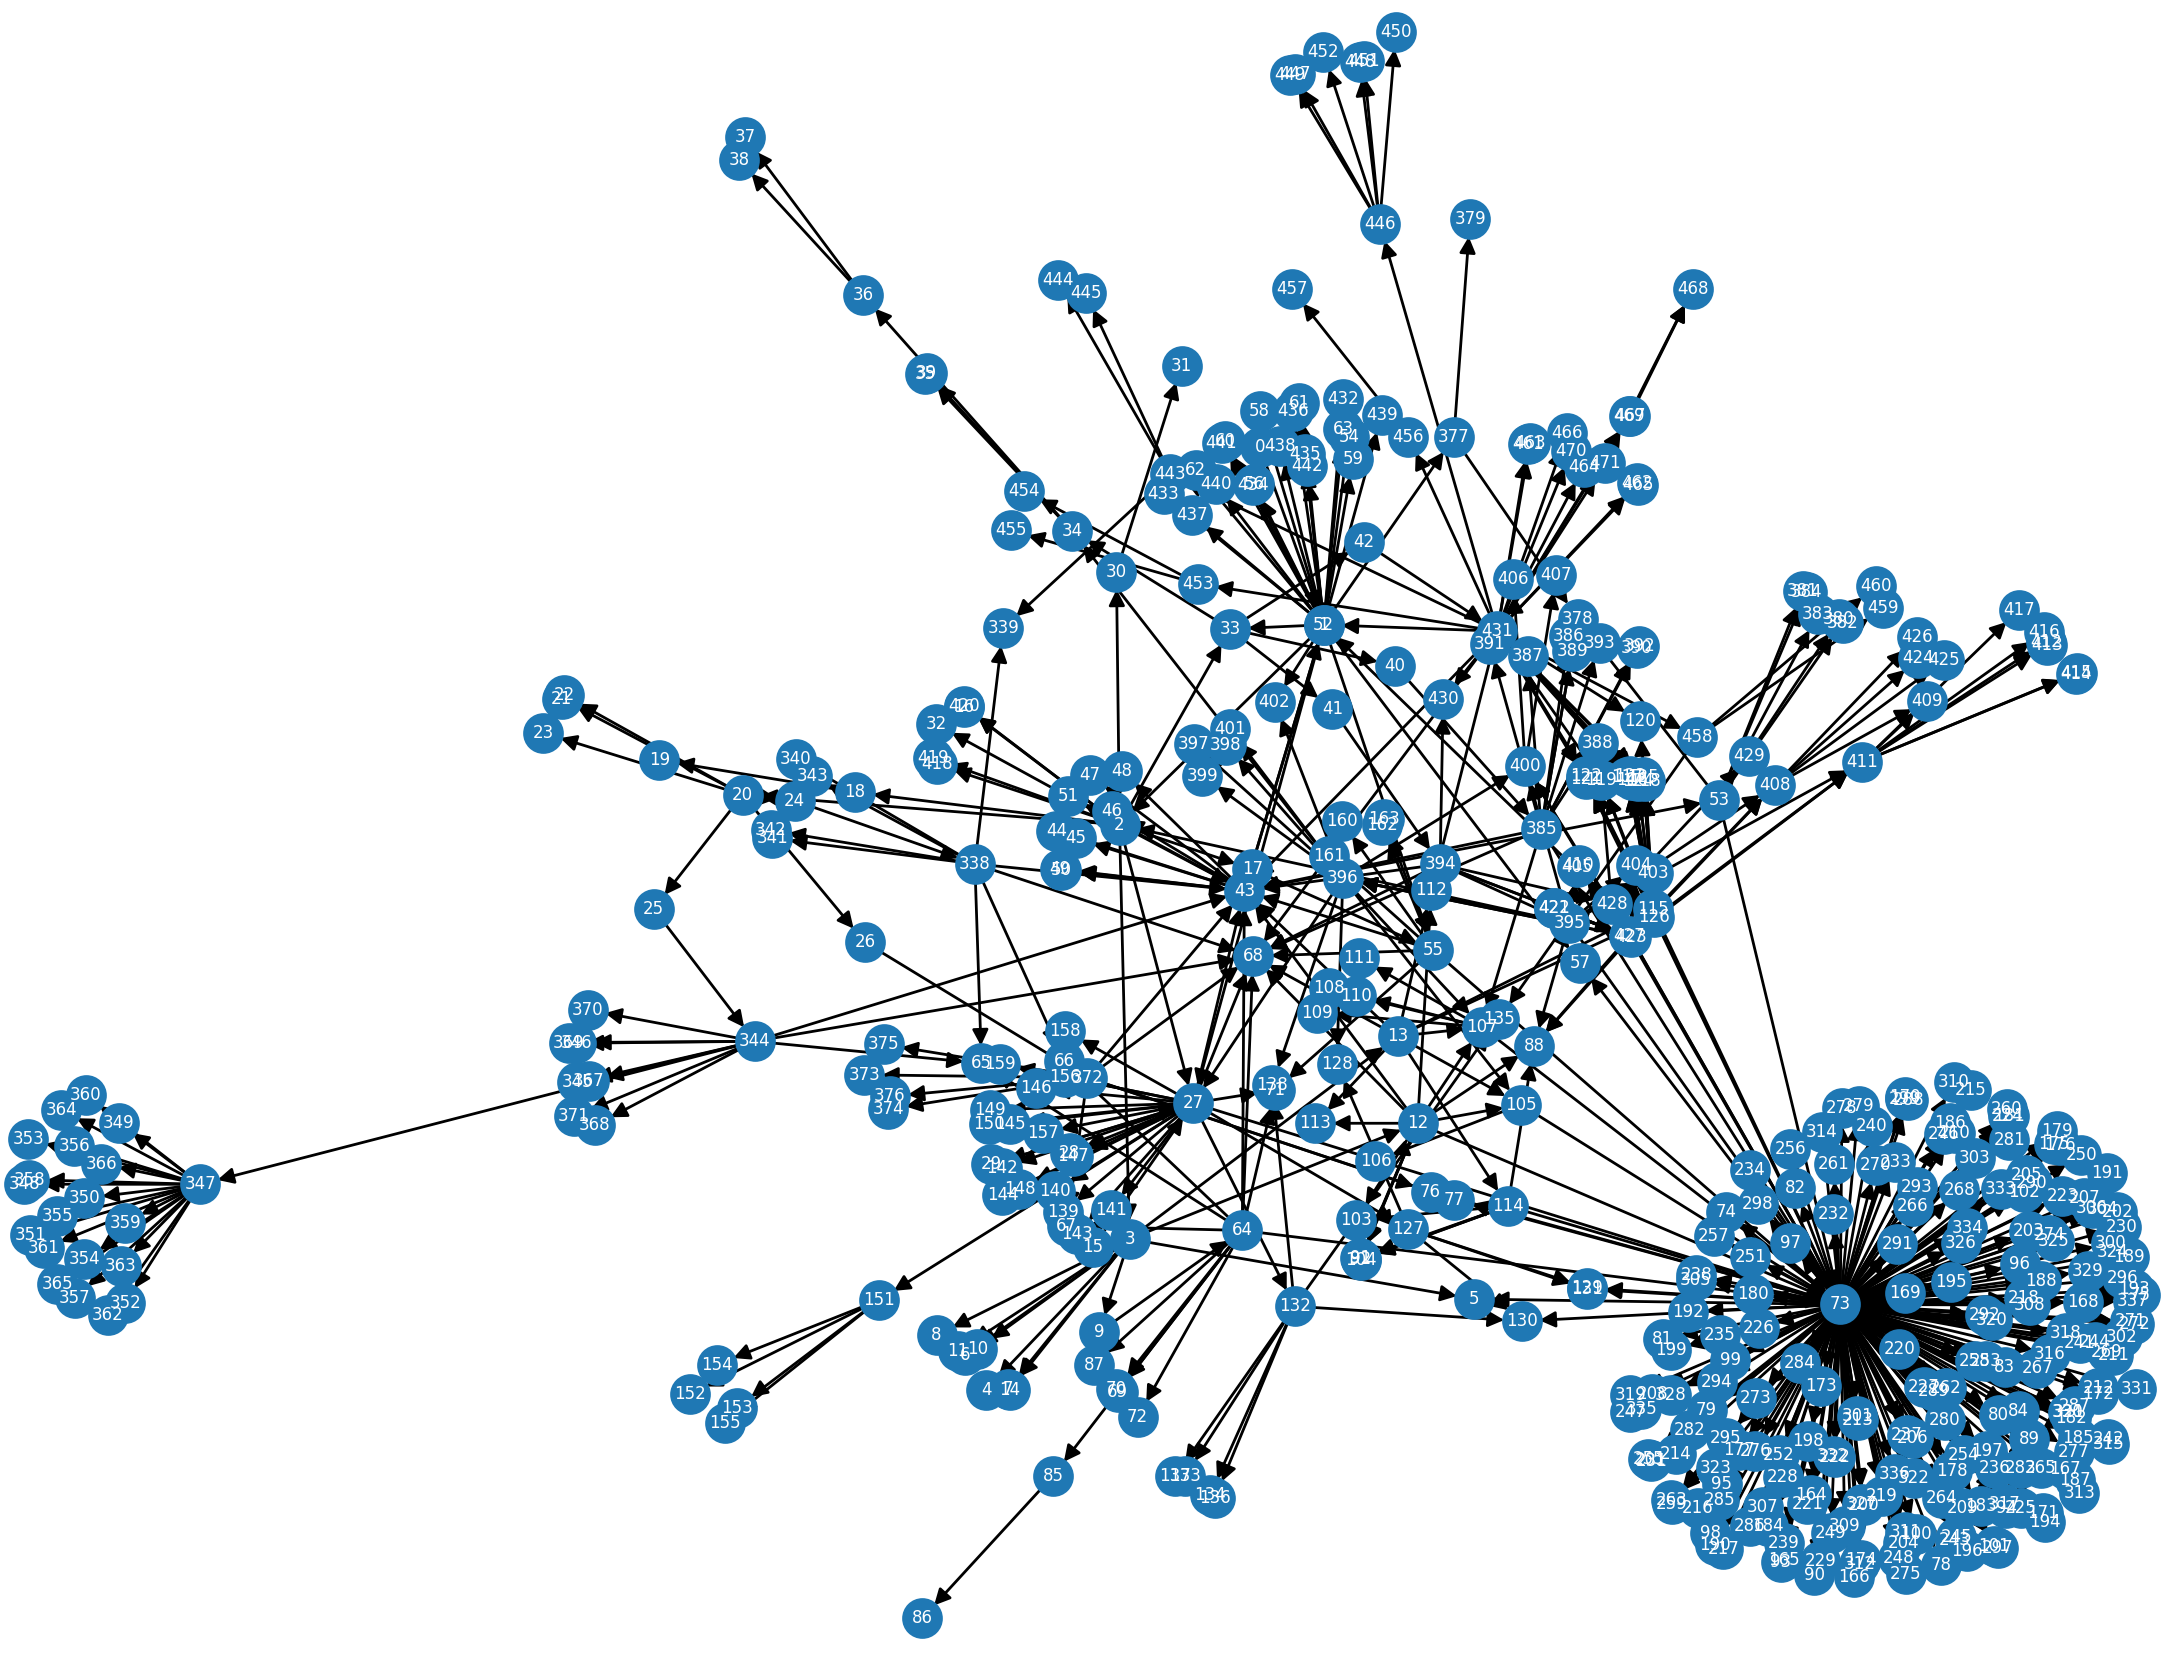
\includegraphics[width=0.85\textwidth,clip]{obrazky-figures/libreoffice_n_end.png}
	\caption{Final event flow graph of LibreOffice StartCenter}
	\label{libreoffice-graph2}
\end{figure}

%window detection, spawning application withing - changing window
%bug found
\section{Comparison with Existing Test Suites}
As discussed in Chapter \ref{proposed_solution}, the approach to application testing done by this work combines several testing techniques and takes advantage of existing testing frameworks and libraries. To the best of my knowledge, there is no tool currently available that tries to achieve the same goal, targeted on applications built for the GNOME environment. The closest related solutions were described in Section \ref{TEMA_TOOLSET}. However, the solution is designed for applications with different development cycles, where a model is being developed before a prototype of the application is available. Other solutions (e.g. references \cite{ReisJacinto2018Aetw},\cite{ArltS2012LSAf}) rely on static analysis and build a model from the source codes of the GUI applications written in Java. The proposed solution derives the model of the SUT from the metadata provided by the accessibility.

When it comes to solutions used for the test automation for GNOME applications, several record and replay tools were described in Section \ref{record_replay}. The proposed solution utilizes \textit{dogtail} combined with framework \textit{behave}, so the generated test cases are executable even after the generation process is finished.

Scripted test cases are written by humans (testers). Their goal is either to automate scenarios that cover key features in applications or to create scenarios based on previously discovered bugs and defects. However, the proposed test generator is a semi-smart tool. Errors and crashes that occur during the generation process are recognized and reported with a reproducer. The potential problem is with the semantics of the test cases. The test generator can apply a sequence of actions to the application although it cannot decide whether the outcome is expected. Therefore, the proposed tool should aid the testers with the development of the test automation right after the executable version of an application is available. The main advantage is in the exploratory testing performed during the test generation. The test generator can sequentially execute available events (test sequences) and possibly help testers to avoid drawbacks of manual testing. The report from the test generation process will also point out the widgets that were not covered by the exploratory testing and therefore they are not covered by the test cases. An additional benefit is provided by the fairly quick availability of the working test automation. Testers can push either all or a subset of test cases in the CI environment. Any test case can be reviewed and updated, new test cases could be written with available \textit{behave} steps or a new step definition can be added. Generated test cases can be merged with the test automation available from the previous versions, if it is not too obsolete.

The test generator itself is a piece of software as well. It is designed to work with as many applications as possible, therefore, the implementation is as general as possible. If a tested application reveals flaws that may be fixed within the test generator. The fixes must maintain the approach that the implementation has to be as general as possible, thus they will not affect the other components. Therefore, if the fix is too application-specific, the effort that needs to be done to include the fix in the test generator should not be greater than developing a custom test case.

In conclusion, generated test cases are not comparable with the currently available test automation developed by testers with script-based tools. The goal of generated test cases is to cover as many events in applications as possible whereas the currently available test suites are focused on automation of the most essential tasks performed by users in which bugs and defects occurred in the past. This comparison does not include unit tests or any other white-box tests performed on the library level.


\chapter{Conclusion}
